\documentclass[a4paper, 10pt]{extarticle}
\usepackage[margin=1in]{geometry}
\usepackage{amsfonts, amsmath, amssymb}
%\usepackage[none]{hyphenat}
\usepackage{fancyhdr} %create a custom header and footer
\usepackage[utf8]{inputenc}
\usepackage[english, main=ukrainian]{babel}
\usepackage{pgfplots}
\usepgfplotslibrary{fillbetween,colormaps}
\usepackage{bm}
\usepackage{float}
\usepackage{physics}
\usepackage[unicode]{hyperref}
\usepackage{scalerel,stackengine}
\usepackage{amsthm}
\usepackage{tikz-cd}
\usetikzlibrary{calc,patterns,angles,quotes, matrix}

\usepackage{tikz-3dplot}
\usetikzlibrary{fit,matrix}

\fancyhead{}
\fancyfoot{}
\parindent 0ex
\def\huge{\displaystyle}
\def\defin#1{\textbf{Definition {#1}}}
\def\ex#1{\textbf{Example {#1}}}
\def\rm#1{\textbf{Remark {#1}}}
\def\prp#1{\textbf{Proposition {#1}}}
\def\lm#1{\textbf{Lemma {#1}}}
\def\th#1{\textbf{Theorem {#1}}}
\def\crl#1{\textbf{Corollary {#1}}}
\def\proof{\textbf{Proof.}\\}
\def\proofMI{\textbf{Proof MI.}\\}
\def\bigline{\vspace{5mm}\\}
\def\qed{$\blacksquare$}
\def\dim#1{\textrm{dim} {#1}}
\def\ker#1{\textrm{Ker} {#1}}
\def\contra{\textbf{!}}

\def\qed{$\blacksquare$}

\def\rightproof{$\boxed{\Rightarrow}$ }
\def\leftproof{$\boxed{\Leftarrow}$ }

\def\noProof{\\ \textit{Без доведення.}}

\newtheoremstyle{theoremdd}% name of the style to be used
  {\topsep}% measure of space to leave above the theorem. E.g.: 3pt
  {\topsep}% measure of space to leave below the theorem. E.g.: 3pt
  {\normalfont}% name of font to use in the body of the theorem
  {0pt}% measure of space to indent
  {\bfseries}% name of head font
  {}% punctuation between head and body
  { }% space after theorem head; " " = normal interword space
  {\thmname{#1}\thmnumber{ #2}\textnormal{\thmnote{ \textbf{#3}\\}}}

\theoremstyle{theoremdd}
\newtheorem{theorem}{Theorem}[subsection]
  
\theoremstyle{theoremdd}
\newtheorem{definition}[theorem]{Definition}

\theoremstyle{theoremdd}
\newtheorem{samedef}[theorem]{Definition}

\theoremstyle{theoremdd}
\newtheorem{example}[theorem]{Example}

\theoremstyle{theoremdd}
\newtheorem{proposition}[theorem]{Proposition}

\theoremstyle{theoremdd}
\newtheorem{remark}[theorem]{Remark}

\theoremstyle{theoremdd}
\newtheorem{lemma}[theorem]{Lemma}

\theoremstyle{theoremdd}
\newtheorem{corollary}[theorem]{Corollary}

\makeatletter
\renewenvironment{proof}[1][Proof.\\]{\par
\pushQED{\hfill \qed}%
\normalfont \topsep6\p@\@plus6\p@\relax
\trivlist
\item\relax
{\bfseries
#1\@addpunct{.}}\hspace\labelsep\ignorespaces
}{%
\popQED\endtrivlist\@endpefalse
}
\makeatother

\newenvironment{pfMI}{\vspace*{-3mm} \textbf{\\ Proof MI. \\}}{\hfill $\blacksquare$}
\newenvironment{pfNoTh}{\textbf{Proof. \\}}{$\blacksquare$}

\DeclareMathOperator{\lcm}{lcm}



\begin{document}
\tableofcontents
\newpage
	
\section{Вектори}
\subsection{Основні означення}
\begin{definition}
\textbf{Вектором} називають напрямлений відрізок.\\
Позначення: $\vec{a}$.
\begin{figure}[h]
\centering
\begin{tikzpicture}
	\draw[thick, ->] (0,0)--(2,1) node at (1,1) {$\vec{a}$};
	\end{tikzpicture}
\end{figure}
\end{definition}

\begin{definition}
Два вектора, що лежать на паралельних прямих (або на одній прямій), називають \textbf{колінеарними}.\\
Позначення: $\vec{a} \parallel \vec{b}$.\\
Інші позначення для колінеарних векторів: \\ 
$\vec{a} \uparrow \uparrow \vec{b}$ - співнапрямлені вектори\\
$\vec{a} \uparrow \downarrow \vec{b}$ - протилежно напрямлені вектори
\bigskip \\
$|\vec{a}|$ - довжина вектора
\end{definition}

\begin{definition}
Вектори $\vec{a}$ та $\vec{b}$ називають \textbf{рівними}, якщо:
	\begin{align*}
	\vec{a} \uparrow \uparrow \vec{b} \\
	|\vec{a}| = |\vec{b}|
	\end{align*}
\end{definition}

\begin{definition}
Задані операції над векторами:\\
	- \textbf{додавання};
\begin{figure}[H]
\centering
	\begin{tikzpicture}
	\draw[thick, ->] (0,0)--(2,2) node at (1,1.5) {$\vec{a}$};
	\draw[thick, ->] (2,2)--(4,2) node at (2.5,2.5) {$\vec{b}$};
	\draw[thick, red, ->] (0,0)--(4,2) node at (2,0.5) {$\vec{a}+\vec{b}$};
	\node at (2,-1) {правило трикутника};
	\end{tikzpicture}
	\qquad
	\begin{tikzpicture}
	\draw[thick, ->] (0,0)--(2,2) node at (1,1.5) {$\vec{a}$};
	\draw[thick, ->] (0,0)--(2,0) node at (1,-0.5) {$\vec{b}$};
	
	\draw[thick, dashed] (2,2)--(4,2);
	\draw[thick, dashed] (2,0)--(4,2);
	\draw[thick, red, ->] (0,0)--(4,2) node at (3,1) {$\vec{a}+\vec{b}$};
	\node at (2,-1) {правило паралелограма};
	\end{tikzpicture}
\end{figure}
	- \textbf{множення на скаляр;}

\begin{figure}[H]
\centering
	\begin{tikzpicture}
	\draw[thick, red, ->] (0,0)--(4,2) node at (3,1) {$\lambda \vec{a}$};
	\draw[thick, ->] (0,0)--(2,1) node at (1,1) {$\vec{a}$};
	\draw[white] (0,-1)--(2,-1);
	\node at (2,-2) {$\lambda > 0$};
	\end{tikzpicture}
	\qquad
	\begin{tikzpicture}
	\draw[thick, red, ->] (0,0)--(-4,-2) node at (-3,-1) {$\lambda \vec{a}$};
	\draw[thick, ->] (0,0)--(2,1) node at (1,1) {$\vec{a}$};
	\draw[white] (0,-1)--(2,-1);
	\node at (-1,-2) {$\lambda < 0$};
	\end{tikzpicture}
\end{figure}
\end{definition}
	Зокрема виконуються ось такі властивості $\forall \vec{a}, \vec{b}, \vec{c}: \forall \lambda, \mu \in \mathbb{R}:$\\
	1) $\vec{a} + \vec{b} = \vec{b} + \vec{a}$
\begin{figure}[H]
\centering
	\begin{tikzpicture}
	\draw[thick, ->] (0,0)--(2,2) node at (1,1.5) {$\vec{a}$};
	\draw[thick, ->] (2,2)--(4,2) node at (2.5,2.5) {$\vec{b}$};
	\draw[thick, red, ->] (0,0)--(4,2) node at (2,0.5) {$\vec{a}+\vec{b}$};
	\end{tikzpicture}
	\qquad
	\begin{tikzpicture}
	\draw[thick, ->] (2,0)--(4,2) node at (2.5,0) {$\vec{a}$};
	\draw[thick, ->] (0,0)--(2,0) node at (1.5,0.5) {$\vec{b}$};
	\draw[thick, red, ->] (0,0)--(4,2) node at (2,1.6) {$\vec{b}+\vec{a}$};
	\end{tikzpicture}
\end{figure}
	2) $(\vec{a} + \vec{b}) + \vec{c} = \vec{a} + (\vec{b} + \vec{c})$
\begin{figure}[H]
\centering
	\begin{tikzpicture}
	\draw[thick, ->] (0,0)--(2,2) node at (1,1.5) {$\vec{a}$};
	\draw[thick, ->] (2,2)--(4,2) node at (2.5,2.5) {$\vec{b}$};
	\draw[thick, ->] (4,2)--(6,1) node at (4.5,1.5) {$\vec{c}$};
	\draw[thick, red, ->] (0,0)--(4,2) node at (3,1) {$\vec{a}+\vec{b}$};
	\draw[thick, blue, ->] (0,0)--(6,1) node at (3,-0.1) {$(\vec{a} + \vec{b}) + \vec{c}$};
	\end{tikzpicture}
	\qquad
	\begin{tikzpicture}
	\draw[thick, ->] (0,0)--(2,2) node at (1,1.5) {$\vec{a}$};
	\draw[thick, ->] (2,2)--(4,2) node at (2.5,2.5) {$\vec{b}$};
	\draw[thick, ->] (4,2)--(6,1) node at (4.5,2.3) {$\vec{c}$};
	\draw[thick, red, ->] (2,2)--(6,1) node at (3,1.3) {$\vec{b}+\vec{c}$};
	\draw[thick, blue, ->] (0,0)--(6,1) node at (3,-0.1) {$\vec{a} + (\vec{b} + \vec{c})$};
	\end{tikzpicture}
\end{figure}
	3) $\exists \vec{0}: \vec{a} + \vec{0} = \vec{a}$\\
	4) $\exists (-\vec{a}): \vec{a} + (-\vec{a}) = \vec{0}$\\
	\textit{Тут малюнок навряд чи знадобиться}
	\bigskip \\
	5) $\lambda(\vec{a}+\vec{b}) = \lambda \vec{a} + \lambda \vec{b}$
\begin{figure}[H]
\centering
	\begin{tikzpicture}[scale = 0.8]
	\draw[thick, ->] (0,0)--(2,2) node at (1,1.5) {$\vec{a}$};
	\draw[thick, dashed] (2,2)--(4,4);
	\draw[thick, ->] (2,2)--(4,2) node at (3.5,2.5) {$\vec{b}$};
	\draw[thick, dashed] (4,4)--(8,4);
	\draw[thick, red, ->] (0,0)--(4,2) node at (2,0.5) {$\vec{a}+\vec{b}$};
	\draw[thick, red, ->, opacity = 0.2] (0,0)--(8,4) node at (5,2) {$\lambda \vec{a}+ \lambda \vec{b}$};
	\end{tikzpicture}
	\qquad
	\begin{tikzpicture}[scale = 0.8]
	\draw[thick, ->, opacity = 0.2] (0,0)--(2,2) node at (1,1.5) {$\vec{a}$};
	\draw[thick, ->] (0,0)--(4,4) node at (2.5,3) {$\lambda \vec{a}$};
	\draw[thick, ->, opacity = 0.2] (2,2)--(4,2) node at (3.5,2.5) {$\vec{b}$};
	\draw[thick, ->] (4,4)--(8,4) node at (6,4.5) {$\lambda \vec{b}$};
	\draw[thick, red, ->, opacity = 0.2] (0,0)--(4,2) node at (2,0.5) {$\vec{a}+\vec{b}$};
	\draw[thick, red, ->] (0,0)--(8,4) node at (5,2) {$\lambda \vec{a}+ \lambda \vec{b}$};
	\end{tikzpicture}
\end{figure}
	\textit{Випливає із подібності трикутників}\\
	6) $\vec{a} (\lambda + \mu) = \lambda \vec{a} + \mu \vec{a}$\\
	7) $(\lambda \mu) \vec{a} = (\lambda \mu) \vec{a}$\\
	8) $1 \cdot \vec{a} = \vec{a}$\\
	\textit{Тут малюнок навряд чи знадобиться}

\begin{definition}
	Два вектори, що лежать на перпендикулярних прямих, називають \textbf{ортогональними}.\\
Позначення: $\vec{a} \perp \vec{b}$.
\end{definition}

\subsection{Поняття базис}
\begin{proposition}
$\vec{a} \parallel \vec{b} \iff \exists \lambda \in \mathbb{R}: \vec{a} = \lambda \vec{b}$.
\end{proposition}

\begin{proof}
$\vec{a} \parallel \vec{b} \iff \left[ \begin{gathered} \vec{a} \uparrow \uparrow \vec{b} \\ \vec{a} \uparrow \downarrow \vec{b} \end{gathered} \right. \iff \exists \lambda: \left[ \begin{gathered} \vec{a} = \underset{=\lambda}{\dfrac{|\vec{a}|}{|\vec{b}|}} \vec{b} \\ \vec{a} = \underset{=\lambda}{-\dfrac{|\vec{a}|}{|\vec{b}|}} \vec{b} \end{gathered} \right.$\\
Ці значення $\lambda$ отримали з огляду на відношення двох "відрізків".
\end{proof}

\begin{remark}
$\vec{0} \parallel \vec{b}$ для будь-якого $\vec{b}$.
\end{remark}

\subsubsection{Випадок на площині}
\begin{theorem}
Задані два вектори $\vec{a}$, $\vec{b}$, що не колінеарні. Тоді $\forall \vec{c}$ на площині: $\exists! \alpha, \beta \in \mathbb{R}:$\\
$\vec{c} = \alpha \vec{a} + \beta \vec{b}$.
\end{theorem}

\begin{proof}
	Маємо довільні вектори $\vec{a}$, $\vec{b}$, $\vec{c}$ на площині. Ми перемістимо їх, щоб лежали на одному спільному початку
\begin{figure}[H]
\centering
	\begin{tikzpicture}
	\draw[thick, ->] (0,0)--(1,1) node at (1,1.5) {$\vec{a}$};
	\draw[thick, dashed] (2,2)--(0,0) node [anchor = south] {$A$};
	\draw[thick, ->] (0,0)--(-2,0) node at (-1,-0.5) {$\vec{b}$};
	\draw[thick, dashed] (0,0)--(2,0)  node [anchor = south] {$D$};
	\draw[thick, red, ->] (0,0)--(4,2) node at (2,1.5) {$\vec{c}$};
	\draw[thick, dashed] (2,0)--(4,2) node [anchor = south] {$C$};
	\draw[thick, dashed] (4,2)--(2,2) node [anchor = south] {$B$};
	\end{tikzpicture}
\end{figure}
	Вздовж векторів $\vec{a}$, $\vec{b}$ ми також провели заштриховані лінії для зручності.\\
\textit{Існування.}\\
	Із малюнку видно, що $\vec{c} = \overrightarrow{AC} = \overrightarrow{AB} + \overrightarrow{AD}$.\\
	Також з малюнку зауважимо, що $\left. \begin{gathered} \overrightarrow{AD} \parallel \vec{b} \\ \overrightarrow{AB} \parallel \vec{a} \end{gathered} \right. \overset{\textrm{\textbf{Prp. 1.2.1.}}}{\Rightarrow} \exists \alpha, \beta: \left. \begin{gathered} \overrightarrow{AD} = \beta \vec{b} \\ \overrightarrow{AB} = \alpha \vec{a} \end{gathered} \right.$.\\
	Отже, $\vec{c} = \alpha \vec{a} + \beta \vec{b}$.
\bigskip \\
\textit{Єдиність.}\\
!Припустимо, що розклад не є єдиним, тобто $\exists \alpha', \beta': \vec{c} = \alpha' \vec{a} + \beta' \vec{b}$.\\
	Тоді $\vec{0} = \vec{c} - \vec{c} = (\alpha-\alpha') \vec{a} + (\beta - \beta') \vec{b}$.\\
	$\implies (\alpha-\alpha')\vec{a} = (\beta' - \beta)\vec{b} \overset{\textrm{\textbf{Prp. 1.2.1.}}}{\Rightarrow} \vec{a} \parallel \vec{b}$.\\
	Але за умовою теореми, $\vec{a} \not\parallel \vec{b}$. Суперечність!\\ Тому та рівність виконується лише при $\alpha = \alpha'$, $\beta = \beta'$, що й доводить єдиність.
\end{proof}

\begin{definition}
\textbf{Базисом на площині} будемо називати фіксовану пару неколінеарних векторів $\vec{a},\vec{b}$.\\
Уже довели, що кожний вектор $\vec{c}$ виражається через базисні вектори як $\vec{c} = \alpha \vec{a} + \beta \vec{b}$ - це \textbf{розклад за базисом}.\\
А коефіцієнти $\alpha$, $\beta$ задають \textbf{координати}.
\end{definition}
	
\subsubsection{Випадок в просторі}
\begin{definition}
Три вектори в просторі називаються \textbf{компланарними}, якщо вони паралельні одній площині.
\end{definition}

\begin{proposition}
$\vec{a}$, $\vec{b}$, $\vec{c}$ - компланарні $\iff \exists \alpha, \beta, \gamma \in \mathbb{R}: \alpha \vec{a} + \beta \vec{b} + \gamma \vec{c} = \vec{0}$.
\end{proposition}

\begin{proof}
	\rightproof Дано: $\vec{a}$, $\vec{b}$, $\vec{c}$ - компланарні. Тоді перемістимо ці вектори так, щоб лежали на одній площині. Тоді один з векторів розкладається за базисом при $\vec{a} \not\parallel \vec{b} \implies \vec{c} = \alpha \vec{a} + \beta \vec{b}$.\\
	$\implies \exists \alpha, \beta, \gamma = -1: \alpha \vec{a} + \beta \vec{b} + \gamma \vec{c} = \vec{0}$.\\
	Якщо ж $\vec{a} \parallel \vec{b}$, то $\vec{a} = \lambda \vec{b}\implies \exists \alpha = 1, \beta = -\lambda, \gamma = 0: \alpha \vec{a} + \beta \vec{b} + \gamma \vec{c} = \vec{0}$.
	\bigskip \\
	\leftproof Дано: $\exists \alpha, \beta, \gamma \in \mathbb{R}: \alpha \vec{a} + \beta \vec{b} + \gamma \vec{c} = \vec{0}$.\\
	Не втрачаючи загальності, нехай $\gamma \neq 0$. Тоді звідси отримаємо:\\
	$\vec{c} = \left( -\dfrac{\alpha}{\gamma} \right) \vec{a} + \left( -\dfrac{\beta}{\gamma} \right) \vec{b}$ - розклад за базисом на площині. Отже, $\vec{c}$ на одній площині з $\vec{a},\vec{b}$, тому вони є компланарними.
\end{proof}

\begin{theorem}
Задані вектори $\vec{a}$, $\vec{b}$, $\vec{c}$, що не компланарні. Тоді $\forall \vec{d}$ в просторі: $\exists! \alpha, \beta, \gamma \in \mathbb{R}:$\\
	$\vec{d} = \alpha \vec{a} + \beta \vec{b} + \gamma \vec{c}$.
\end{theorem}

\begin{proof}
	Маємо довільні вектори $\vec{a}$, $\vec{b}$, $\vec{c}$, $\vec{d}$ в просторі. Ми перемістимо їх, щоб лежали на одному спільному початку.
\begin{figure}[H]
\centering
	\begin{tikzpicture}
    % Axes
    %\draw [->] (0,0,0) -- (3,0,0) node [right] {$x$};
    %\draw [->] (0,0,0) -- (0,3,0) node [left] {$y$};
    %\draw [->] (0,0,0) -- (0,0,3) node [left] {$z$};
    \draw[thick, red, ->] (2,0,2)--(0,2,0) node[anchor = south] {$\vec{d}$};
    \draw[thick, ->] (2,0,2)--(3,0,2) node at (3,-0.5,2) {$\vec{a}$};
    \draw[thick, ->] (2,0,2)--(2,0,1) node at (2,0.5,1) {$\vec{b}$};
    \draw[thick, ->] (2,0,2)--(2,1,2) node at (1.8,1.2,2) {$\vec{c}$};
    
    %Construction
    \draw[thick, dashed] (0,0,0)--(2,0,0) node [right] {$B_1$};
    \draw[thick, dashed] (2,0,0)--(2,0,2) node [anchor = north] {$C_1$};
    \draw[thick, dashed] (2,0,2)--(0,0,2) node [left] {$D_1$};
    \draw[thick, dashed] (0,0,2)--(0,0,0) node [left] {$A_1$};
    \draw[thick, dashed] (0,2,0)--(2,2,0) node [right] {$B_2$};
    \draw[thick, dashed] (2,2,0)--(2,2,2) node [right] {$C_2$};
    \draw[thick, dashed] (2,2,2)--(0,2,2) node [left] {$D_2$};
    \draw[thick, dashed] (0,2,2)--(0,2,0) node [left] {$A_2$};
    \draw[thick, dashed] (0,2,0)--(0,0,0);
    \draw[thick, dashed] (2,2,0)--(2,0,0);
    \draw[thick, dashed] (2,2,2)--(2,0,2);
    \draw[thick, dashed] (0,2,2)--(0,0,2);
	\end{tikzpicture}
\end{figure}
	Вздовж векторів $\vec{a}$, $\vec{b}$, $\vec{c}$ ми також провели заштриховані лінії для зручності.\\
	\textit{Існування.}\\
	Із малюнку видно, що $\vec{d} = \overrightarrow{C_1D_1} = \overrightarrow{C_1B_1} + \overrightarrow{C_1C_2}$.\\
	А тепер за порядком, що видно ще на малюнку:\\
	$\overrightarrow{C_1D_1},$ $\vec{a}$ - колінеарні, тому $\overrightarrow{C_1D_1} = \alpha \vec{a}$;\\
	$\overrightarrow{C_1B_1},$ $\vec{b}$ - колінеарні, тому $\overrightarrow{C_1B_1} = \beta \vec{b}$;\\
	$\overrightarrow{C_1C_2},$ $\vec{c}$ - колінеарні, тому $\overrightarrow{C_1C_2} = \gamma \vec{c}$.\\
	Тому $\vec{d} = \alpha \vec{a} + \beta \vec{b} + \gamma \vec{c}$.\\
	А доведення на єдиність є аналогічним до \textbf{Th. 1.2.3.} Тільки ми до суперечності прийдемо від того, що ці вектори стануть компланарними після припущення.
\end{proof}

\begin{definition}
\textbf{Базисом в просторі} будемо називати фіксовану пару некомпланарних векторів $\vec{a}$, $\vec{b}$, $\vec{c}$\\
Уже довели, що кожний вектор $\vec{d}$ виражається через базисні вектори як $\vec{d} = \alpha \vec{a} + \beta \vec{b} + \gamma \vec{c}$ - це \textbf{розклад за базисом}.\\
А коефіцієнти $\alpha$, $\beta$, $\gamma$ задають \textbf{координати}.
\bigskip \\
Ще також в означенні можна позначати $\vec{d} = (\alpha, \beta, \gamma)$ - як набір координат в заданому базисі.
\end{definition}

В обох підпунктах виконується наступне твердження (надалі в основному буду розглядати випадок простору):
\begin{theorem}
Задано базис векторів $\vec{a}$, $\vec{b}$, $\vec{c}$ і вектори $\vec{d_1} = (\alpha_1, \beta_1, \gamma_1)$, $\vec{d_2} = (\alpha_2, \beta_2, \gamma_2)$. Тоді:\\
	1) $\vec{d_1} + \vec{d_2} = (\alpha_1+\alpha_2, \beta_1+\beta_2, \gamma_1+\gamma_2)$;\\
	2) $\lambda \vec{d_1} = (\lambda \alpha_1, \lambda \beta_1, \lambda \gamma_1)$.\\
	\textit{Вказівка: підставити задані вектори та винести за дужки базисні вектори.}
\end{theorem}

\begin{example}
Нехай т. $O$ - точка перетину медіан трикутника $ABC$. Відомо, що $\overrightarrow{AO} = \vec{a}, \overrightarrow{AC} = \vec{b}$. Розкласти вектор $\overrightarrow{AB}$ за базисом $\vec{a}, \vec{b}$.
\begin{figure}[H]
\centering
	\begin{tikzpicture}[scale = 3]
	\draw[thick] (0,0)--(1,1) node[anchor = south] {$A$};
	\draw[thick] (1,1)--(1.5,0) node[anchor = west] {$B$};
	\draw[thick] (1.5,0)--(0,0) node[anchor = east] {$C$};
	\draw[thick] (1,1)--(0.75,0) node[anchor = north] {$D$};
	\draw[fill] ({5/6},{1/3}) circle[radius=0.5 pt] node[anchor = west] {$O$};
	\draw[->, red] (1,1)--({5/6},{1/3}) node at (0.8,0.6) {$\vec{a}$};
	\draw[->, red] (1,1)--(0,0) node at (0.4,0.6) {$\vec{b}$};
	\draw (0.375,-1pt)--(0.375,1pt);
	\draw (1.125,-1pt)--(1.125,1pt);
	\end{tikzpicture}
\end{figure}
	Із малюнку можна сказати, що $\overrightarrow{AB} = \overrightarrow{AC} + \overrightarrow{CB}$.\\
	Перший вектор $\overrightarrow{AC} = \vec{b}$ за умовою задачі. Другий вектор $\overrightarrow{CB} = 2 \overrightarrow{CD}$. Водночас $\overrightarrow{AC} + \overrightarrow{CD} = \overrightarrow{AD}$.\\
	За властивістю медіан трикутників, маємо, що $\dfrac{\abs{\overrightarrow{AO}}}{\abs{\overrightarrow{OD}}} = \dfrac{2}{1}$, тому $\abs{\overrightarrow{OD}} = \dfrac{1}{2} \abs{\overrightarrow{AO}} = \dfrac{1}{2} \abs{\vec{a}}$.\\
	А оскільки вони ще й співнапрямлені, то тоді $\overrightarrow{OD} = \dfrac{1}{2} \vec{a}$.\\
	Звідси $\overrightarrow{AD} = \dfrac{3}{2} \vec{a}$.	Тоді $\overrightarrow{CD} = \overrightarrow{AD} - \overrightarrow{AC} = \dfrac{3}{2} \vec{a} - \vec{b}$.\\
	Остаточно $\overrightarrow{AB} = 3 \vec{a} - \vec{b}$.
\end{example}
	
\subsection{Декартова система координат}
\begin{definition}
Нехай в просторі задано базис $\vec{a}$, $\vec{b}$, $\vec{c}$. Встановимо фіксовану т. $O$ - початок координат, туди й прикладемо всі вектори.\\
Така сукупність називається \textbf{декартовою системою координат.}
\begin{figure}[H]
\centering
	\begin{tikzpicture}
	\draw[fill] (0,0,0) circle[radius=2 pt] node[anchor = north] {$O$};
	\draw[thick, ->] (0,0,0)--(2,0,1) node[anchor = north] {$\vec{a}$};
	\draw[thick, ->] (0,0,0)--(3,2,0) node[anchor = north] {$\vec{b}$};
	\draw[thick, ->] (0,0,0)--(1,3,0) node[anchor = north west] {$\vec{c}$};
	\end{tikzpicture}
\end{figure}
\end{definition}
Будь-якій т. $M$ в просторі однозначно відповідає вектор $\overrightarrow{OM}$ - \textbf{радіус-вектор}.\\
	Розкладемо за нашим базисом:\\
	$\overrightarrow{OM} = \alpha_M \vec{a} + \beta_M \vec{b} + \gamma_M \vec{c} = (\alpha_M, \beta_M, \gamma_M)$.\\
	Через однозначність ми назвемо $M(\alpha_M, \beta_M, \gamma_M)$ \textbf{координатами} т. $M$.
	\bigskip \\
	А тепер нехай задані т. $M(\alpha_M, \beta_M, \gamma_M)$, $N(\alpha_N, \beta_N, \gamma_N)$. Знайдемо координати вектора $\overrightarrow{MN}$.\\
	Враховуючи існування початку координат, отримаємо:\\
	$\overrightarrow{MN} = \overrightarrow{ON} - \overrightarrow{OM} = (\alpha_N - \alpha_M, \beta_N - \beta_M, \gamma_N - \gamma_M)$.
	
	
\subsection{Лінійна залежність/незалежність}
\begin{definition}
Система векторів $\{\vec{a_1}, \dots, \vec{a_n}\}$ називається:\\
	- \textbf{лінійно незалежною}, якщо з рівності $\alpha_1 \vec{a_1} + \dots + \alpha_n \vec{a_n} = \vec{0}$, де $\alpha_1, \dots, \alpha_n \in \mathbb{R}$, випливає $\alpha_1 = \dots = \alpha_n = 0$;\\
	- \textbf{лінійно залежною}, якщо $\exists \alpha_1, \dots, \alpha_n \in \mathbb{R}: |\alpha_1| + \dots + |\alpha_n| \neq 0: \alpha_1 \vec{a_1} + \dots + \alpha_n \vec{a_n} = \vec{0}$.
\end{definition}

\begin{definition}
Вираз $\alpha_1 \vec{a_1} + \dots + \alpha_n \vec{a_n}$, де $\alpha_1, \dots, \alpha_n \in \mathbb{R}$, називається \textbf{лінійною комбінацією}.
\end{definition}

\begin{proposition}
$\{\vec{a}$, $\vec{b}\}$ - лінійно залежна $\iff \vec{a} \parallel \vec{b}$.
\end{proposition}

\begin{proof}
	$\{\vec{a},\vec{b}\}$ - лінійно залежна $\iff$ $\exists \alpha, \beta: |\alpha| + |\beta| \neq 0: \alpha \vec{a} + \beta \vec{b} = \vec{0} \boxed{\iff}$\\
	Не втрачаючи загальності, ми вважатимемо, що $\alpha \neq 0$.\\
	$\boxed{\iff} \vec{a} = -\dfrac{\beta}{\alpha} \vec{b} \overset{\text{позн.} \lambda = -\frac{\beta}{\alpha}}{=} \lambda \vec{b} \iff \vec{a} \parallel \vec{b}$.
\end{proof}

\begin{corollary}
$\{\vec{a}, \vec{b}\}$ - лінійно незалежні $\iff \vec{a} \not\parallel \vec{b}$.
\end{corollary}

\begin{proposition}
	На площині будь-які три вектори завжди лінійно залежні.
\end{proposition}

\begin{proof}
	Розглянемо вектори $\{\vec{a},\vec{b},\vec{c}\}$. І знову, не втрачаючи загальності, візьмемо перші два вектори та розглянемо два підпункти:\\
	I. $\vec{a} \parallel \vec{b}$.\\
	Тоді $\vec{a} = \lambda \vec{b} \implies 1 \cdot \vec{a} + (-\lambda) \vec{b} + 0 \cdot \vec{c} = \vec{0}$, причому тут $|1|+|-\lambda|+|0| \neq 0$. Отже, $\{\vec{a}, \vec{b}, \vec{c}\}$ - лінійно залежна.
	\bigskip \\
	II. $\vec{a} \not\parallel \vec{b}$.\\
	Тоді $\exists \alpha, \beta: \vec{c} = \alpha \vec{a} + \beta \vec{b} \implies \alpha \vec{a} + \beta \vec{b} + (-1) \vec{c} = \vec{0}$, причому тут $|\alpha| + |\beta| + |-1| \neq 0$. Отже, $\{\vec{a}, \vec{b}, \vec{c}\}$ - лінійно залежна.\\
	Остаточно маємо, що 3 вектори на площині - лінійно залежні.
\end{proof}

\begin{proposition}
$\{\vec{a},\vec{b},\vec{c} \}$ - лінійно залежні $\iff$ $\vec{a},\vec{b},\vec{c}$ - компланарні.
\end{proposition}

\begin{proof}
	$\{\vec{a},\vec{b},\vec{c}\}$ - лінійно залежні $\iff \exists \alpha, \beta, \gamma: |\alpha| + |\beta| + |\gamma| \neq 0: \alpha \vec{a} + \beta \vec{b} + \gamma \vec{c} = \vec{0} \boxed{\iff}$\\
	Не обмежуючи загальності, нехай $\alpha \neq 0$.\\
$\boxed{\iff} \vec{a} = -\dfrac{\beta}{\alpha} \vec{b} - \dfrac{\gamma}{\alpha} \vec{c} \overset{\textrm{позн.} \lambda = -\frac{\beta}{\alpha}, \mu = -\frac{\gamma}{\alpha}}{=} \lambda \vec{b} + \mu \vec{c} \iff$ $\vec{a},\vec{b},\vec{c}$ - компланарні.
\end{proof}

\begin{corollary}
	$\{\vec{a},\vec{b},vec{c}\}$ - лінійно незалежні $\iff$ $\vec{a},\vec{b},\vec{c}$ - не компланарні.
\end{corollary}

\begin{proposition}
	В просторі будь-які чотири вектори завжди лінійно залежні.
\end{proposition}

\begin{proof}
	Розглянемо вектори $\{\vec{a},\vec{b},vec{c},\vec{d}\}$. І знову не втрачаючи загальності, візьмемо перші три вектори та розглянемо два підпункти:\\
	I. $\vec{a}$, $\vec{b}$, $\vec{c}$ - компланарні.\\
	Тоді $\exists \alpha, \beta: \vec{c} = \alpha \vec{a} + \beta \vec{b} \implies \alpha \vec{a} + \beta \vec{b} + (-1)\vec{c} + 0 \cdot \vec{d} = \vec{0}$, причому тут $|\alpha| + |\beta| + |-1| + |0| \neq 0$. Отже, $\{\vec{a}, \vec{b}, \vec{c}, \vec{d}\}$ - лінійно залежна.
	\bigskip \\
	II. $\vec{a}$, $\vec{b}$, $\vec{c}$ - не компланарні.\\
	Тоді $\exists \alpha, \beta, \gamma: \vec{d} = \alpha \vec{a} + \beta \vec{b} + \gamma \vec{c} \implies \alpha \vec{a} + \beta \vec{b} + \gamma \vec{c} + (-1)\vec{d} = \vec{0}$, причому тут $|\alpha| + |\beta| + |\gamma| + |-1| \neq 0$. Отже, $\{\vec{a}, \vec{b}, \vec{c}, \vec{d}\}$ - лінійно залежні.\\
	Остаточно маємо, що 4 вектори в просторі - лінійно залежні.
\end{proof}

\begin{corollary}
	У просторі вектори кількістю більше 4 завжди лінійно залежні.
\end{corollary}
	
\subsection{Проєкція на вісь}
\begin{definition}
	\textbf{Проєкцією вектора $\vec{a}$ на вісь $l$} називають вираз:
	\begin{align*}
	pr_l \vec{a} = \pm |AB|
	\end{align*}
	Якщо $\vec{a}$ утворює гострий кут з віссю $l$, то беремо знак +.\\
	Якщо $\vec{a}$ утворює тупий кут з віссю $l$, то беремо знак -.
\begin{figure}[H]
\centering
	\begin{tikzpicture}
	\draw[thick, ->] (0,0)--(4,0) node[right] {$l$};
	\draw[thick, ->] (1,1)--(3,2) node[anchor = south east] {$\vec{a}$};
	\draw[thick, dashed] (1,0)--(1,1); \draw[thick, dashed] (3,0)--(3,2);
	\draw (1,-1pt)--(1,1pt) node [anchor = north] {$A$};
	\draw (3,-1pt)--(3,1pt) node [anchor = north] {$B$};
	\draw[very thick, red] (1,0)--(3,0);
	\draw[thick, dashed] (1,1)--(2,1);
	\draw[thick] (1.75,1) arc (0:atan(1/2):0.75) node [anchor = west] {$\alpha$};
	\end{tikzpicture}
\end{figure}
\end{definition}

	Якщо перемістити паралельно $\vec{a}$ так, щоб початок був в т. $A$, то маємо з малюнку:\\
	$|AB| = |\vec{a}| \cos \alpha$.\\
	Ця формула буде також справедливою при розгляданні тупого кута.\\
	Отримали інакшу формулу проєкції:
	\begin{align*}
	pr_l \vec{a} = |\vec{a}| \cos \alpha
	\end{align*}
	
\begin{proposition}[Властивості]
	1) $pr_l (\vec{a} + \vec{b}) = pr_l \vec{a} + pr_l \vec{b}$\\
	2) $pr_l (\lambda \vec{a}) = \lambda \cdot pr_l \vec{a}$\\
\end{proposition}

\begin{proof}
	1) Тут є чотири випадки, наведу ілюстративно.
\begin{figure}[H]
\centering
	\begin{tikzpicture}
	%axis
	\draw[thick, ->] (0,0)--(5,0) node[right] {$l$};
	
	%vectors
	\draw[thick, ->] (1,1)--(3,2) node at (2,1.2) {$\vec{a}$};
	\draw[thick, ->] (3,2)--(4,3) node at (4.2,2.5) {$\vec{b}$};
	\draw[thick, red, ->] (1,1)--(4,3) node[anchor = south east] {$\vec{a} + \vec{b}$};
	
	%projection
	\draw[thick, dashed] (1,0)--(1,1); \draw[thick, dashed] (3,0)--(3,2); \draw[thick, dashed] (4,0)--(4,3);
	\draw (1,-1pt)--(1,1pt) node [anchor = north] {$A$};
	\draw (3,-1pt)--(3,1pt) node [anchor = north] {$C$};
	\draw (4,-1pt)--(4,1pt) node [anchor = north] {$B$};
	\end{tikzpicture}
	\qquad
	\begin{tikzpicture}
	%axis
	\draw[thick, ->] (0,0)--(5,0) node[right] {$l$};
	
	%vectors
	\draw[thick, ->] (1,1)--(3,2) node at (2.3,1.2) {$\vec{a}$};
	\draw[thick, ->] (3,2)--(2,3) node at (3.2,2.5) {$\vec{b}$};
	\draw[thick, red, ->] (1,1)--(2,3) node[anchor = south east] {$\vec{a} + \vec{b}$};
	
	%projection
	\draw[thick, dashed] (1,0)--(1,1); \draw[thick, dashed] (3,0)--(3,2); \draw[thick, dashed] (2,0)--(2,3);
	\draw (1,-1pt)--(1,1pt) node [anchor = north] {$A$};
	\draw (3,-1pt)--(3,1pt) node [anchor = north] {$C$};
	\draw (2,-1pt)--(2,1pt) node [anchor = north] {$B$};
	\end{tikzpicture}
\end{figure}

\begin{figure}[H]
\centering
	\begin{tikzpicture}
	%axis
	\draw[thick, ->] (0,0)--(5,0) node[right] {$l$};
	
	%vectors
	\draw[thick, ->] (4,1)--(2,2) node at (2.5,1.5) {$\vec{a}$};
	\draw[thick, ->] (2,2)--(3,3) node at (2,2.5) {$\vec{b}$};
	\draw[thick, red, ->] (4,1)--(3,3) node[anchor = south east] {$\vec{a} + \vec{b}$};
	
	%projection
	\draw[thick, dashed] (4,0)--(4,1); \draw[thick, dashed] (2,0)--(2,2); \draw[thick, dashed] (3,0)--(3,3);
	\draw (4,-1pt)--(4,1pt) node [anchor = north] {$A$};
	\draw (2,-1pt)--(2,1pt) node [anchor = north] {$C$};
	\draw (3,-1pt)--(3,1pt) node [anchor = north] {$B$};

	\end{tikzpicture}
	\qquad
	\begin{tikzpicture}
	%axis
	\draw[thick, ->] (0,0)--(5,0) node[right] {$l$};
	
	%vectors
	\draw[thick, ->] (4,1)--(2,2) node at (2.5,1.5) {$\vec{a}$};
	\draw[thick, ->] (2,2)--(1,3) node at (1.5,2) {$\vec{b}$};
	\draw[thick, red, ->] (4,1)--(1,3) node[anchor = south] {$\vec{a} + \vec{b}$};
	
	%projection
	\draw[thick, dashed] (4,0)--(4,1); \draw[thick, dashed] (2,0)--(2,2); \draw[thick, dashed] (1,0)--(1,3);
	\draw (4,-1pt)--(4,1pt) node [anchor = north] {$A$};
	\draw (2,-1pt)--(2,1pt) node [anchor = north] {$C$};
	\draw (1,-1pt)--(1,1pt) node [anchor = north] {$B$};
	\end{tikzpicture}
\end{figure}
	1.1) $pr_l (\vec{a} +\vec{b}) = |AB|  = |AC| + |CB| = pr_l \vec{a} + pr_l \vec{b}$.\\
	1.2), 1.3), 1.4) аналогічно.
	\bigline
	2) Тут теж чотири випадки, знову ілюстративно.
\begin{figure}[H]
\centering
	\begin{tikzpicture}
%axis
	\draw[thick, ->] (0,0)--(5,0) node[right] {$l$};
	
	%vectors
	\draw[thick, red, ->] (2,1.5)--(4,2.5) node at (3,2.5) {$\lambda \vec{a}$};
	\draw[thick, ->] (2,1.5)--(3,2) node at (2.5,1.5) {$\vec{a}$};
	
	%projection
	\draw[thick, dashed] (2,0)--(2,1.5); \draw[thick, dashed] (3,0)--(3,2); \draw[thick, dashed] (4,0)--(4,2.5);
	\draw (2,-1pt)--(2,1pt) node [anchor = north] {$A$};
	\draw (3,-1pt)--(3,1pt) node [anchor = north] {$C$};
	\draw (4,-1pt)--(4,1pt) node [anchor = north] {$B$};
	\end{tikzpicture}
	\qquad
	\begin{tikzpicture}
%axis
	\draw[thick, ->] (0,0)--(5,0) node[right] {$l$};
	
	%vectors
	\draw[thick, red, ->] (2,1.5)--(1,1) node at (1.2,1.5) {$\lambda \vec{a}$};
	\draw[thick, ->] (2,1.5)--(3,2) node at (2.5,1.5) {$\vec{a}$};
	
	%projection
	\draw[thick, dashed] (2,0)--(2,1.5); \draw[thick, dashed] (3,0)--(3,2); \draw[thick, dashed] (1,0)--(1,1);
	\draw (2,-1pt)--(2,1pt) node [anchor = north] {$A$};
	\draw (3,-1pt)--(3,1pt) node [anchor = north] {$C$};
	\draw (1,-1pt)--(1,1pt) node [anchor = north] {$B$};
	\end{tikzpicture}
\end{figure}

\begin{figure}[H]
\centering
\begin{tikzpicture}
%axis
	\draw[thick, ->] (0,0)--(5,0) node[right] {$l$};
	
	%vectors
	\draw[thick, red, ->] (3,2)--(1,1) node at (1.2,1.5) {$\lambda \vec{a}$};
	\draw[thick, ->] (3,2)--(2,1.5) node at (2.5,1.5) {$\vec{a}$};
	
	%projection
	\draw[thick, dashed] (3,0)--(3,2); \draw[thick, dashed] (2,0)--(2,1.5); \draw[thick, dashed] (1,0)--(1,1);
	\draw (3,-1pt)--(3,1pt) node [anchor = north] {$A$};
	\draw (2,-1pt)--(2,1pt) node [anchor = north] {$C$};
	\draw (1,-1pt)--(1,1pt) node [anchor = north] {$B$};
	\end{tikzpicture}
\qquad
\begin{tikzpicture}
%axis
	\draw[thick, ->] (0,0)--(5,0) node[right] {$l$};
	
	%vectors
	\draw[thick, red, ->] (3,2)--(4,2.5) node at (3,2.5) {$\lambda \vec{a}$};
	\draw[thick, ->] (3,2)--(2,1.5) node at (2.5,1.5) {$\vec{a}$};
	
	%projection
	\draw[thick, dashed] (3,0)--(3,2); \draw[thick, dashed] (2,0)--(2,1.5); \draw[thick, dashed] (4,0)--(4,2.5);
	\draw (3,-1pt)--(3,1pt) node [anchor = north] {$A$};
	\draw (2,-1pt)--(2,1pt) node [anchor = north] {$C$};
	\draw (4,-1pt)--(4,1pt) node [anchor = north] {$B$};
	\end{tikzpicture}
\end{figure}
	2.1) $pr_l (\lambda \vec{a}) = |AB| = \dfrac{|AB|}{|AC|} |AC| = \lambda pr_l \vec{a}$.\\
	Дріб дорівнює нашому скаляру, використовуючи подібності трикутників (якщо вісь $l$ перемістити до початку $\vec{a}$).\\
	2.2), 2.3), 2.4) аналогічно.
\end{proof}

\begin{definition}
	\textbf{Проєкцією вектора $\vec{a}$ на вектор $\vec{b}$} називають проєкцію вектора на вісь, напрямок якого задається вектором $\vec{b}$.
\end{definition}
	
\subsection{Скалярний добуток}
\begin{definition}
	\textbf{Скалярним добутком векторів $\vec{a}$, $\vec{b}$} називають величину:
	\begin{align*}
	(\vec{a}, \vec{b}) = |\vec{a}| \cdot |\vec{b}| \cdot \cos \alpha,
	\end{align*}
	де $\alpha$ - кут між векторами $\vec{a}$ та $\vec{b}$.
\end{definition}

\begin{proposition}[Критерій ортогональності]
	$\vec{a} \perp \vec{b} \iff (\vec{a}, \vec{b}) = 0$.
\end{proposition}

\begin{proof}
Тут ми розгладатимемо ненульові вектори $\vec{a},\vec{b}$. Бо в тому випадку нецікаво.\\
	$(\vec{a}, \vec{b}) = 0 \iff |\vec{a}| |\vec{b}| \cos \alpha = 0 \iff \cos \alpha = 0 \iff \vec{a} \perp \vec{b}$.
\end{proof}

\begin{proposition}[Властивості]
	1) $(\vec{a}, \vec{b}) = (\vec{b}, \vec{a})$\\
	2) $(\vec{a}, \vec{b}) = pr_{\vec{b}} \vec{a} \cdot |\vec{b}| = pr_{\vec{a}} \vec{b} \cdot |\vec{a}|$\\
	3) $(\vec{a_1}+\vec{a_2}, \vec{b}) = (\vec{a_1}, \vec{b}) + (\vec{a_2}, \vec{b})$\\
	4) $(\lambda \vec{a}, \vec{b}) = \lambda (\vec{a}, \vec{b})$\\
	5) $(\vec{a}, \vec{a}) = |\vec{a}|^2$\\
	6) $\forall \vec{b}: (\vec{a}, \vec{b}) = 0 \implies \vec{a} = \vec{0}$\\
	7) $\forall \vec{d}: (\vec{a}, \vec{d}) = (\vec{b}, \vec{d}) \implies \vec{a} = \vec{b}$
\end{proposition}

\begin{proof}
	1) $(\vec{a}, \vec{b}) = |\vec{a}| |\vec{b}| \cos \alpha = |\vec{b}| |\vec{a}| \cos \alpha = (\vec{b}, \vec{a})$ \bigskip \\
	2) $(\vec{a}, \vec{b}) = |\vec{a}| |\vec{b}| \cos \alpha = pr_{\vec{b}} \vec{a} \cdot |\vec{b}| = pr_{\vec{a}} \vec{b} \cdot |\vec{a}|$ \bigskip \\
	3) $(\vec{a_1}+\vec{a_2}, \vec{b}) = pr_{\vec{b}} (\vec{a_1} + \vec{a_2}) |\vec{b}| = pr_{\vec{b}} \vec{a_1} |\vec{b}| + pr_{\vec{b}} \vec{a} |\vec{b}| = (\vec{a_1}, \vec{b}) + (\vec{a_2}, \vec{b})$ \bigskip \\
	4) $(\lambda \vec{a}, \vec{b}) = pr_{\vec{b}} (\lambda \vec{a}) |\vec{b}| = \lambda pr_{\vec{b}} (\vec{a}) |\vec{b}| = \lambda (\vec{a}, \vec{b})$ \bigskip \\
	5) $(\vec{a}, \vec{a}) = |\vec{a}| |\vec{a}| \cos 0 = |\vec{a}|^2$\bigskip \\
	6) $\forall \vec{b}: (\vec{a}, \vec{b}) = 0 \overset{\vec{b} = \vec{a}}{\implies} (\vec{a}, \vec{a}) = 0 \implies \vec{a} = \vec{0}$ \bigskip \\
	7) $\forall \vec{d}: (\vec{a}, \vec{d}) = (\vec{b}, \vec{d}) \implies (\vec{a}-\vec{b}, \vec{d}) = (\vec{a}, \vec{d}) - (\vec{b}, \vec{d}) = 0 \implies \vec{a} - \vec{b} = 0 \implies \vec{a} = \vec{b}$
\end{proof}

\begin{example}
	Нехай задані такі вектори $\vec{a}, \vec{b}$, що $|\vec{a}| = 3, |\vec{b}| = 2$, а також кут між ними становить $\dfrac{2 \pi}{3}$. З'ясувати, чи будуть вектори $\vec{a}+2 \vec{b}$ та $3 \vec{a} - \vec{b}$ ортогональними.
	Для цього знайдемо їхній скалярний добуток.
	За властивістю скалярного добутку, маємо:\\
	$(\vec{a} + 2 \vec{b}, 3 \vec{a} - \vec{b}) = 3 (\vec{a}, \vec{a}) - (\vec{a}, \vec{b}) + 6 (\vec{b}, \vec{a}) - 2 (\vec{b}, \vec{b}) = 3 |\vec{a}|^2 + 5 (\vec{a}, \vec{b}) - 2 |\vec{b}|^2 = 27 + 5 |\vec{a}| |\vec{b}| \cos \dfrac{2 \pi}{3} - 8 = 4$\\
	$(\vec{a} + 2 \vec{b}, 3 \vec{a} - \vec{b}) \neq 0 \Rightarrow \vec{a} + 2 \vec{b} \not\perp 3 \vec{a} - \vec{b}$
\end{example}

	Розглянемо вектори $\vec{a} = (a_1, a_2, a_3), \vec{b} = (b_1, b_2, b_3)$, які розкладені за деяким базисом $\{\vec{p}, \vec{q}, \vec{r}\}$. Знайдемо скалярний добуток цих векторів $\vec{a},\vec{b}$:\\
	$(\vec{a}, \vec{b}) = (a_1\vec{p} + a_2\vec{q} + a_3\vec{r}$ , $b_1\vec{p} + b_2\vec{q} + b_3\vec{r}) = \\
	a_1 b_1 (\vec{p}, \vec{p}) + a_1 b_2 (\vec{p}, \vec{q}) + a_1 b_3 (\vec{p}, \vec{r}) + 
	+ a_2 b_1 (\vec{q}, \vec{p}) + a_2 b_2 (\vec{q}, \vec{q}) + a_2 b_3 (\vec{q}, \vec{r}) + 
	+ a_3 b_1 (\vec{r}, \vec{p}) + a_3 b_2 (\vec{r}, \vec{q}) + a_3 b_3 (\vec{r}, \vec{r})$.\\
	Поки нічого особливого. Проте якщо ми вимагатимемо, щоб $\vec{p} \perp \vec{q}$, $\vec{q} \perp \vec{r}$, $\vec{r} \perp \vec{p}$, то \\
	$(\vec{p}, \vec{q}) = (\vec{q}, \vec{r}) = (\vec{r}, \vec{p}) = 0$.
	
\begin{definition}
	Базис, в якому всі вектори перпендикулярні між собою, називається \textbf{ортогональним}.
\end{definition}

	Тоді отримаємо такий вираз:\\
	$(\vec{a}, \vec{b}) = a_1 b_1 |\vec{p}|^2 + a_2 b_2 |\vec{q}|^2 + a_3 b_3 |\vec{r}|^2$.\\
	Уже формула приємніше. Але буде краще, коли додамо умову, щоб $\vec{p}$, $\vec{q}$, $\vec{r}$ будуть одиничними, тобто $|\vec{p}| = |\vec{q}| = |\vec{r}| = 1$.
	
\begin{definition}
	Ортогональний базис, в якому довжина векторів одинична, називається \textbf{ортонормальним}.\\
	Позначення: $\{\vec{i}, \vec{j}, \vec{k}\}$.
\end{definition}

\begin{remark}
	Надалі ми будемо мати справу саме з цим ортонормованим базисом.
\end{remark}

	Остаточно отримаємо:
\begin{proposition}
	Для векторів $\vec{a} = (a_1, a_2, a_3), \vec{b} = (b_1, b_2, b_3)$ в ортонормованому базисі скалярний добуток рахується таким чином:\\
	$(\vec{a}, \vec{b}) = a_1 b_1 + a_2 b_2 + a_3 b_3$.
\end{proposition}

\begin{corollary}
	Для векторів $\vec{a} = (a_1, a_2, a_3)$ в ортонормованому базисі\\
	$|\vec{a}| = \sqrt{a_1^2 + a_2^2 + a_3^2}$.
\end{corollary}

\subsection{Векторний добуток векторів}
\begin{definition}
	Упорядковану трійку некомпланарних векторів $\vec{a}, \vec{b}, \vec{c}$ ми будемо називати \textbf{правою}, якщо сісти на кінець вектора $\vec{c}$, взяти менший з кутів між $\vec{a}$ та $\vec{b}$ та спостерігати поворот від $\vec{a}$ до $\vec{b}$ \textit{проти годинникової} стрілки

\begin{figure}[H]
\centering
\tdplotsetmaincoords{60}{120}
\begin{tikzpicture}[tdplot_main_coords]
\draw[thick,->] (0,0,0) -- (2,0,0) node[anchor=north east]{$\vec{a}$};
\draw[thick,->] (0,0,0) -- (0,2,0) node[anchor=north west]{$\vec{b}$};
\draw[thick,->] (0,0,0) -- (1,0,2) node[anchor=south]{$\vec{c}$};
\draw[->] (1,0,0) arc (0:90:1);
\end{tikzpicture}
\end{figure}
\end{definition}

\begin{definition}
	Якщо спостерігаємо це явище \textit{за годинниковою} стрілкою, то тоді впорядковану трійку називають \textbf{лівою}.
\begin{figure}[H]
\centering
\tdplotsetmaincoords{60}{120}
\begin{tikzpicture}[tdplot_main_coords]
\draw[thick,->] (0,0,0) -- (2,0,0) node[anchor=north east]{$\vec{a}$};
\draw[thick,->] (0,0,0) -- (0,2,0) node[anchor=north west]{$\vec{b}$};
\draw[thick,->] (0,0,0) -- (-1,0,-2) node[anchor=north]{$\vec{c}$};
\draw[->] (1,0,0) arc (0:90:1);
\end{tikzpicture}
\end{figure}
\end{definition}

\begin{proposition}[Властивості]
	Задано праву трійку $\{\vec{a}, \vec{b}, \vec{c}\}$. Тоді:\\
	1) $\{\vec{b}, \vec{c}, \vec{a}\}, \{\vec{c}, \vec{a}, \vec{b}\}$ - права трійка;\\
	2) $\{\vec{a}, \vec{b}, -\vec{c}\}, \{-\vec{a}, \vec{b}, -\vec{c}\}, \{\vec{a}, -\vec{b}, -\vec{c}\}$ - ліва трійка;\\
	3) $\{\vec{b}, \vec{a}, \vec{c}\}, \{\vec{a}, \vec{c}, \vec{b}\}, \{\vec{c}, \vec{b}, \vec{a}\}$ - ліва трійка.\\
	\textit{Випливає з геометричних міркувань.}
\end{proposition}

\begin{definition}
	\textbf{Векторним добутком векторів $\vec{a}, \vec{b}$} називають вектор $\vec{c}$, який:\\
	1) $|\vec{c}| = |\vec{a}| |\vec{b}| \sin \alpha$, $\alpha$ - кут між вектором $\vec{a}$ та $\vec{b}$;\\
	2) $\vec{c} \perp \vec{a}, \vec{c} \perp \vec{b}$;\\
	3) $\{\vec{a}, \vec{b}, \vec{c}\}$ - права трійка.
\begin{figure}[H]
\centering
\tdplotsetmaincoords{60}{120}
\begin{tikzpicture}[tdplot_main_coords]
\draw[thick,->] (0,0,0) -- (2,0,0) node[anchor=north east]{$\vec{a}$};
\draw[thick,->] (0,0,0) -- (0,2,0) node[anchor=north west]{$\vec{b}$};
\draw[thick,->] (0,0,0) -- (0,0,2) node[anchor=south]{$\vec{c}$};
\draw[->] (1,0,0) arc (0:90:1) node at (1,1,0) {$\alpha$};
\draw[thick] (0,0,0.5)--(0,0.5,0.5)--(0,0.5,0);
\draw[thick] (0,0,0.5)--(0.5,0,0.5)--(0.5,0,0);
\end{tikzpicture}
\end{figure}
Позначення: $\vec{c} = [\vec{a}, \vec{b}]$.
\end{definition}

\begin{proposition}[Властивості]
1) $[\vec{a}, \vec{b}] = -[\vec{b}, \vec{a}]$\\
2) $[\vec{a}, \vec{b}] = \vec{0} \iff \vec{a} \parallel \vec{b}$\\
3) $[\vec{a_1} + \vec{a_2}, \vec{b}] = [\vec{a_1}, \vec{b}] + [\vec{a_2}, \vec{b}]$\\
4) $[\lambda \vec{a}, \vec{b}] = \lambda [\vec{a}, \vec{b}]$
\end{proposition}

\begin{proof}
1) $|[\vec{b}, \vec{a}]| = |[\vec{a}, \vec{b}]| = |\vec{a}| |\vec{b}| \sin \alpha$\\
За означенням, $[\vec{a}, \vec{b}]$ та $[\vec{b}, \vec{a}]$ одночасно $\perp \vec{a}$, $\perp \vec{b}$. Звідси випливає (із геометрії), що
$[\vec{a}, \vec{b}] \parallel [\vec{b}, \vec{a}] \implies [\vec{a}, \vec{b}] = \pm [\vec{b}, \vec{a}]$.\\
Коли $\{\vec{b}, \vec{a}, [\vec{b}, \vec{a}]\}$ - права, то $\{\vec{a}, \vec{b}, [\vec{b}, \vec{a}]\}$ - ліва, а тому $\{\vec{a}, \vec{b}, -[\vec{b}, \vec{a}]\}$ - права. Отже, $[\vec{b},\vec{a}] = -[\vec{a}, \vec{b}]$.
\bigskip \\
2) Тут ми розглядатимемо ненульові вектори $\vec{a},\vec{b}$. Бо в тому випадку нецікаво.\\
$[\vec{a}, \vec{b}] = \vec{0} \iff |[\vec{a}, \vec{b}]| = 0 \iff |\vec{a}| |\vec{b}| \sin \alpha = 0 \iff \alpha = 0,\pi \iff \vec{a} \parallel \vec{b}$.
\bigskip \\
3), 4) на потім залишемо. Хоча залишу інший варіант.\\
\textit{Альтернативне доведення.}\\
Зробимо ось такий геометричний малюнок. Векторний добуток $[\vec{a_1},\vec{b}]$ відповідатиме блакитній грані. Векторний добуток $[\vec{a_2},\vec{b}]$ відповідатиме зеленій грані. Нарешті, векторний добуток $[\vec{a_1}+\vec{a_2}, \vec{b}]$ відповідатиме останній грані.
\begin{figure}[H]
\centering
\begin{tikzpicture}
\filldraw[draw=black, fill=white] (0,0)--(3,0.5)--(2.5,2)--(-0.5,1.5)--cycle;
\filldraw[draw=black, fill=blue!10] (0,0)--(1,1)--(0.5,2.5)--(-0.5,1.5)--cycle;
\filldraw[draw=black, fill=green!10] (3,0.5)--(1,1)--(0.5,2.5)--(2.5,2)--cycle;
\draw[dashed] (2.5,2)--(-0.5,1.5);

\draw[thick,->] (0,0)--(-0.5,1.5) node[anchor = east] {$\vec{b}$};
\draw[thick,blue,->] (0,0)--(1,1) node[anchor = north] {$\vec{a_1}$};
\draw[thick,green,->] (1,1)--(3,0.5) node[anchor = west] {$\vec{a_2}$};
\draw[thick,red,->] (0,0)--(3,0.5) node[anchor = north east] {$\vec{a_1}+\vec{a_2}$};
\end{tikzpicture}
\end{figure}
Я поки припущу, що $\vec{a_1},\vec{a_2}$ утворюють трикутник при сумуванні.\\
Кожна грань - це паралелограм. Проведемо на кожній грані висоту таким чином, щоб із цих сторін утворити трикутник (цей трикутник буде прямокутним, але щось не можу пояснити). Намалюю якийсь трикутник, щоб було простіше. Одразу позначу довжини сторін.
\begin{figure}[H]
\centering
\begin{tikzpicture}
\draw[red] (0,0)--(3,0);
\draw[green] (3,0)--(2,1);
\draw[blue] (2,1)--(0,0);
\node at (1.5,-0.5) {$|\vec{a_1}+\vec{a_2}| \cos \theta$};
\node at (0,0.7) {$|\vec{a_1}| \cos \varphi_1$};
\node at (3.5,0.7) {$|\vec{a_2}| \cos \varphi_2$};
\end{tikzpicture}
\end{figure}
$\varphi_1$ - кут між $\vec{a_1}, \vec{b}$.\\
$\varphi_2$ - кут між $\vec{a_2}, \vec{b}$.\\
$\theta$ - кут між $\vec{a_1}+\vec{a_2}, \vec{b}$.\\
За теоремою Піфагора, маємо $|\vec{a_1}|^2 \cos^2 \varphi_1 + |\vec{a_2}|^2 \cos^2 \varphi_2 = |\vec{a_1}+\vec{a_2}|^2 \cos^2 \theta$.\\
Помножимо обидві частини рівності на $|\vec{b}|^2$:\\
$|\vec{a_1}|^2 |\vec{b}|^2 \cos^2 \varphi_1 + |\vec{a_2}|^2 |\vec{b}|^2 \cos^2 \varphi_2 = |\vec{a_1}+\vec{a_2}|^2 |\vec{b}|^2 \cos^2 \theta$ (*).\\
Зауважимо тепер, що $[\vec{a_1},\vec{b}]$ перпендикулярний синій стороні, $[\vec{a_2},\vec{b}]$ перпендикулярний зеленій стороні, $[\vec{a_1}+\vec{a_2},\vec{b}]$ перпендикулярний червоній стороні.\\
Якщо на $90^\circ$ повернути малюнок з трикутником за годинниковою стрілкою, то ці векторні добутки будуть лежати на цих сторонах. Їх можна об'єднати, просто тому що виконується рівність (*).
\end{proof}

\begin{remark}[Геометричний зміст]
Із означення випливає, що модуль векторного добутку описує площу паралелограма, тобто:\\
$S_{\text{паралелограм}} = |[\vec{a},\vec{b}]|$.
\begin{figure}[H]
\centering
\begin{tikzpicture}
\draw[name path = A, thick,->] (0,0,0) -- (3,0,0) node[anchor=north east]{$\vec{a}$};
\draw[thick,->] (0,0,0) -- (0,3,0) node[anchor=north west]{$\vec{c}$};
\draw[name path = B, thick,->] (0,0,0) -- (0,0,3) node[anchor=south]{$\vec{b}$};
\draw[name path = C, thick, dashed] (0,0,2)--(2,0,2)--(2,0,0);
\fill [blue!50,
    intersection segments={
      of= B and C
    }];
\draw[->] (0.6,0,0) arc [start angle=0,end angle=-90,x radius=0.8,y radius=0.24] node [anchor = north west] {$\alpha$} node[black] at (1,0,0) {$S$};
\draw[thick] (0,0,0.5)--(0,0.5,0.5)--(0,0.5,0);
\draw[thick] (0.5,0,0)--(0.5,0.5,0)--(0,0.5,0);
\end{tikzpicture}
\end{figure}
\end{remark}

\subsection{Мішаний добуток векторів}
\begin{definition}
\textbf{Мішаним добутков трьох векторів $\vec{a}, \vec{b}, \vec{c}$} називають число:
\begin{align*}
(\vec{a}, \vec{b}, \vec{c}) = (\vec{a}, [\vec{b}, \vec{c}])
\end{align*}
Тобто тут скалярний добуток $\vec{a}$ з векторним добутком $\vec{b},\vec{c}$.
\end{definition}

\begin{proposition}[Властивості]
1) Знак мішаного добутку:\\
+, якщо $\{\vec{a}, \vec{b}, \vec{c}\}$ - права трійка\\
-, якщо $\{\vec{a}, \vec{b}, \vec{c}\}$ - ліва трійка\\
2) $(\vec{a}, \vec{b}, \vec{c}) = (\vec{b}, \vec{c}, \vec{a}) = (\vec{c}, \vec{a}, \vec{b}) = -(\vec{b}, \vec{a}, \vec{c}) = -(\vec{a}, \vec{c}, \vec{b}) = -(\vec{c}, \vec{b}, \vec{a})$\\
3) $(\vec{a}, \vec{b}, \vec{c}) = 0 \iff \vec{a}, \vec{b}, \vec{c}$ - компланарні\\
4) $(\vec{a}, \vec{b}, \vec{c}) = (\vec{a}, [\vec{b}, \vec{c}]) = ([\vec{a},\vec{b}],\vec{c})$\\
5) $(\vec{a_1}+\vec{a_2}, \vec{b}, \vec{c}) = (\vec{a_1},\vec{b},\vec{c}) + (\vec{a_2},\vec{b},\vec{c})$\\
6) $(\lambda \vec{a}, \vec{b}, \vec{c}) = \lambda (\vec{a},\vec{b},\vec{c})$
\end{proposition}

\begin{proof}
1) $(a,b,c) > 0 \iff pr_{[\vec{b}, \vec{c}]} \vec{a} > 0 \iff$ кут між цими векторами - гострий $\iff \{\vec{a}, \vec{b}, \vec{c}\}$ - права.\\
$(a,b,c) < 0 \iff pr_{[\vec{b}, \vec{c}]} \vec{a} < 0 \iff$ кут між цими векторами - тупий $\iff \{\vec{a}, \vec{b}, \vec{c}\}$ - ліва.
\bigskip \\
2) Дивись \textbf{Prp. 1.7.3.}, яка трійка: права та ліва. А далі користуємось властивістю 1), щойно доведеною. Тому й виникають рівності.\bigskip \\
3) $(\vec{a}, \vec{b}, \vec{c}) = 0 \iff V = 0$ (див. зауваження нижче), тобто ці вектори лежать на одній площині - компланарні. \bigskip \\
4) $(\vec{a}, [\vec{b},\vec{c}]) = (\vec{a}, \vec{b}, \vec{c}) = (\vec{c}, \vec{a}, \vec{b}) = (\vec{c}, [\vec{a}, \vec{b}]) = ([\vec{a},\vec{b}], \vec{c})$ \bigskip \\
5) $(\vec{a_1}+\vec{a_2}, \vec{b}, \vec{c}) = (\vec{a_1}+\vec{a_2}, [\vec{b},\vec{c}]) = (\vec{a_1},[\vec{b},\vec{c}]) + (\vec{a_2},[\vec{b},\vec{c}]) = (\vec{a_1},\vec{b},\vec{c}) + (\vec{a_2},\vec{b},\vec{c})$\bigskip \\
6) $(\lambda \vec{a}, \vec{b}, \vec{c}) = (\lambda \vec{a}, [\vec{b}, \vec{c}]) = \lambda (\vec{a},[\vec{b},\vec{c}]) = \lambda (\vec{a},\vec{b},\vec{c})$
\end{proof}

\begin{remark}[Геометричний зміст]
Із означення та геометричного сенсу векторного добутку випливає, що мішаний добуток описує об'єм паралелепіпеда, тобто:\\
$V_{\text{паралелепіпед}} = |(\vec{a},\vec{b},\vec{c})|$.
\begin{figure}[H]
\centering
\begin{tikzpicture}
\draw[thick,->] (0,0,0) -- (2,0,2) node[anchor=north east]{$\vec{c}$};
\draw[thick,->] (0,0,0) -- (2,0,-2) node[anchor=south]{$\vec{b}$};
\draw[thick,->] (0,0,0) -- (1,2,0) node[anchor=south]{$\vec{a}$};
\draw[thick, dashed] (1,2,0)--(1,0,0) node at (1.2,1,0) {$h$};
\draw[thick,dashed] (2,0,2) -- (4,0,0) -- (2,0,-2) node at (2,0,0) {$S_{\textrm{осн}}$};
\draw[thick, dashed] (2,0,2)--(3,2,2);
\draw[thick, dashed] (4,0,0)--(5,2,0);
\draw[thick, dashed] (2,0,-2)--(3,2,-2);
\draw[thick, dashed] (3,2,2)--(5,2,0)--(3,2,-2)--(1,2,0)--cycle;
\end{tikzpicture}
\end{figure}
Справді, $V = S\cdot h = |[\vec{b}, \vec{c}]| \cdot |pr_{[\vec{b}, \vec{c}]} \vec{a}| = |[\vec{b}, \vec{b}] pr_{[\vec{b}, \vec{c}]} \vec{a}| = |(\vec{a}, [\vec{b}, \vec{c}])| = |(\vec{a},\vec{b},\vec{c})|$.
\end{remark}

\textbf{Повернміось до п. 1.7.}\\
Доведемо останні два пункти:\\
3) Візьмемо довільний вектор $\vec{d}$ і знайдемо наступний скалярний добуток:\\
$(\vec{d}, [\vec{a_1}+\vec{a_2}, \vec{b}]) = (\vec{d}, \vec{a_1}+\vec{a_2}, \vec{b}) = (\vec{d}, \vec{a_1}, \vec{b}) + (\vec{d}, \vec{a_2}, \vec{b}) = \\ = (\vec{d}, [\vec{a_1}, \vec{b}]) + (\vec{d}, [\vec{a_2}, \vec{b}]) = (\vec{d}, [\vec{a_1},\vec{b}]+[\vec{a_2},\vec{b}])$\\
$\Rightarrow [\vec{a_1}+\vec{a_2}, \vec{b}] = [\vec{a_1},\vec{b}]+[\vec{a_2},\vec{b}]$
\bigskip \\
4) Візьмемо довільний вектор $\vec{d}$ і знайдемо наступний скалярний добуток:\\
$(\vec{d}, [\lambda \vec{a}, \vec{b}]) = (\vec{d}, \lambda \vec{a}, \vec{b}) = \lambda (\vec{d}, \vec{a}, \vec{b}) = \lambda (\vec{d}, [\vec{a}, \vec{b}]) = (\vec{d}, \lambda [\vec{a}, \vec{b}])$\\
$\Rightarrow [\lambda \vec{a}, \vec{b}] = \lambda [\vec{a}, \vec{b}]$ \qed
\bigskip \\
Розглянемо вектори $\vec{a} = (a_1,a_2,a_3), \vec{b} = (b_1,b_2,b_3)$, які розкладені за ортонормованим базисом\\
Знайдемо їхній векторний добуток:\\
$[\vec{a}, \vec{b}] = [a_1\vec{i}+a_2\vec{j}+a_3\vec{k}, b_1\vec{i}+b_2\vec{j}+b_3\vec{k}] = \\ a_1 b_1 [\vec{i}, \vec{i}] + a_1 b_2 [\vec{i}, \vec{j}] + a_1 b_3 [\vec{i}, \vec{k}] + a_2 b_1 [\vec{j}, \vec{i}] + a_2 b_2 [\vec{j}, \vec{j}] + a_2 b_3 [\vec{j}, \vec{k}] + a_3 b_1 [\vec{k}, \vec{i}] + a_3 b_2 [\vec{k}, \vec{j}] + a_3 b_3 [\vec{k}, \vec{k}] = \\
= (a_2 b_3 - a_3 b_2) \vec{i} + (a_1 b_3 - a_3 b_1) \vec{j} + (a_1 b_2 - a_2 b_1) \vec{k} = \begin{vmatrix}
\vec{i} & \vec{j} & \vec{k} \\
a_1 & a_2 & a_3 \\
b_1 & b_2 & b_3
\end{vmatrix}$.\\
Координати вектора $[\vec{a}, \vec{b}] = \left(\begin{vmatrix} a_2 & b_2 \\ a_3 & b_3 \end{vmatrix}, \begin{vmatrix} a_1 & b_1 \\ a_3 & b_3 \end{vmatrix}, \begin{vmatrix} a_1 & b_1 \\ a_2 & b_2 \end{vmatrix} \right)$.\\
Тут ще про визначники ми нычого не говорили, але хотілось цю формулу залишити в компактному вигляді.
\bigskip \\
\textbf{Повернімось до п. 1.8.}\\
Розглянемо вектори $\vec{a} = (a_1,a_2,a_3), \vec{b} = (b_1,b_2,b_3), \vec{c} = (c_1,c_2,c_3)$, які розкладені за ортонормованим базисом. Знайдемо їхній мішаний добуток:\\
$(\vec{a}, \vec{b}, \vec{c}) = ([\vec{a}, \vec{b}], \vec{c}) = c_1 \begin{vmatrix} a_2 & b_2 \\ a_3 & b_3 \end{vmatrix} + c_2 \begin{vmatrix} a_1 & b_1 \\ a_3 & b_3 \end{vmatrix} + c_3 \begin{vmatrix} a_1 & b_1 \\ a_2 & b_2 \end{vmatrix} = \begin{vmatrix}
a_1 & a_2 & a_3 \\
b_1 & b_2 & b_3 \\
c_1 & c_2 & c_3
\end{vmatrix}$

\subsection{Подвійний векторний добуток}
\begin{definition}
\textbf{Подвійним векторним добутком векторів $\vec{a}, [\vec{b},\vec{c}]$} називається вектор:
\begin{align*}
\vec{d} = [\vec{a},[\vec{b},\vec{c}]]
\end{align*}
Позначення: $\vec{d} = [\vec{a},\vec{b},\vec{c}]$.
\end{definition}

\begin{proposition}
$[\vec{a},[\vec{b},\vec{c}]] = \vec{b} (\vec{a}, \vec{c}) - \vec{c} (\vec{a}, \vec{b})$.\\
\textit{Розмновна формула: бац мінус цаб :)}
\end{proposition}

\begin{proof}
Розглянемо вектори $\vec{a} = (a_1, a_2, a_3), \vec{b} = (b_1,b_2,0), \vec{c} = (c_1,0,0)$, які розкладені за ортонормованим базисом. Маємо тоді, що $[\vec{b}, \vec{c}] = (0,0,-b_2 c_1)$.\\
Також $[\vec{a}, [\vec{b}, \vec{c}]] = (-a_2b_2c_1, a_1b_2c_1,0)$.\\
Водночас $\vec{b} (\vec{a}, \vec{c}) - \vec{c} (\vec{a}, \vec{b}) = a_1c_1\vec{b} - (a_1b_1+a_2b_2)\vec{c} = (-a_2b_2c_1,a_1b_2c_1,0)$\\
Отже, $[\vec{a},[\vec{b},\vec{c}]] = \vec{b} (\vec{a}, \vec{c}) - \vec{c} (\vec{a}, \vec{b})$.
\end{proof}

\textit{Альтернативне доведення.}
\begin{figure}[H]
\centering
\begin{tikzpicture}
\draw[name path = A, thick,->] (0,0,0) -- (3,0,1) node[anchor=north east]{$\vec{c}$};
\draw[thick,->] (0,0,0) -- (0,3,0) node[anchor=north west]{$[\vec{b}, \vec{c}]$};
\draw[name path = B, thick,->] (0,0,0) -- (0,0,3) node[anchor=south]{$\vec{b}$};
\draw[thick,->] (0,0,0) -- (1,2,1) node[anchor=north west]{$\vec{a}$};
\end{tikzpicture}
\end{figure}
Розглянемо більш детально подвійні добутки.\\
Спочатку створімо вектор $[\vec{b}, \vec{c}]$. За означенням, $[\vec{b}, \vec{c}] \perp \vec{b},\vec{c}$\\
А потім вже вектор $[\vec{a},\vec{b},\vec{c}]$. За означенням, $[\vec{a},\vec{b},\vec{c}] \perp [\vec{b}, \vec{c}]$.\\
А це означає, що $[\vec{a},\vec{b},\vec{c}]$ лежить на площині, що створена векторами $\vec{b},\vec{c}$, тоді цей вектор розкладемо за базисом: $[\vec{a}, \vec{b}, \vec{c}] = \beta \vec{b} + \gamma \vec{c}$.\\
Залишилось знайти координати $\beta, \gamma$.\\
Нам також відомо, що $[\vec{a},\vec{b},\vec{b}] \perp \vec{a} \implies ([\vec{a}, \vec{b}, \vec{b}], \vec{a}) = 0$.\\
Але з іншого боку, $([\vec{a}, \vec{b}, \vec{b}], \vec{a}) = (\beta \vec{b} + \gamma \vec{c}, \vec{a}) = \beta (\vec{b}, \vec{a}) + \gamma (\vec{c}, \vec{a})$.\\
Таким чином, $(\vec{a}, \vec{b}) \beta + (\vec{a}, \vec{c}) \gamma = 0 \implies \dfrac{\gamma}{(\vec{a}, \vec{b})} = - \dfrac{\beta}{(\vec{a}, \vec{c})} = \lambda$.\\
$\Rightarrow [\vec{a}, \vec{b}, \vec{c}] = -\lambda \vec{b} (\vec{a}, \vec{c}) + \lambda \vec{c} (\vec{a}, \vec{b})$\\
А тепер нехай $\vec{a} = \vec{i}, \vec{b} = \vec{j}, \vec{c} = \vec{i}$. Отримаємо, що\\
$\vec{j} = [\vec{i}, \vec{j}, \vec{i}] = -\lambda \vec{j} \Rightarrow \lambda = -1$.\\
Підставимо це значення та отримаємо $[\vec{a},[\vec{b},\vec{c}]] = \vec{b} (\vec{a}, \vec{c}) - \vec{c} (\vec{a}, \vec{b})$ \qed

\begin{corollary}[Тотожність Якобі]
$[\vec{a}, [\vec{b}, \vec{c}]] + [\vec{b}, [\vec{c}, \vec{a}]] + [\vec{c}, [\vec{a}, \vec{b}]] = \vec{0}$.
\end{corollary}

\subsection{*Формула ділення відрізка в заданому співвідношенні}
Задані точки $A(x_A,y_A,z_A), B(x_B,y_B,z_B)$. Проведемо відрізок $AB$. Встановимо точку $P(x_P,y_P,z_P) \in AB$ таким чином, що $\dfrac{AP}{PB} = \dfrac{\lambda}{\mu}$
\begin{figure}[H]
\centering
\begin{tikzpicture}
\draw[thick] (0,0)--(4,1);
\draw[fill] (0,0) circle (1pt) node [anchor = north]{$A$};
\draw[fill] (1,0.25) circle (1pt) node [anchor = north]{$P$};
\draw[fill] (4,1) circle (1pt) node [anchor = north]{$B$};
\node at (0.5,0.5) {$\lambda$};
\node at (2.5,0.85) {$\mu$};
\end{tikzpicture}
\end{figure}
Знайдемо координати т. $P$.\\
$\dfrac{AP}{PB} = \dfrac{\lambda}{\mu} \implies \mu AP = \lambda PB$.\\
$\overrightarrow{AP} = (x_P - x_A, y_P - y_A, z_P - z_A)$, $\overrightarrow{PB} = (x_B - x_P, y_B - y_P, z_B - z_P)$.\\
$\mu \overrightarrow{AP} = \lambda \overrightarrow{PB}$.\\
Тому $\mu (x_P - x_A) = \lambda (x_B - x_P) \implies \dots \Rightarrow x_P = \dfrac{\lambda x_B + \mu x_A}{\lambda + \mu}$.\\
Для $y_P, z_P$ аналогічна формула.
\newpage

\section{Початок аналітичної геометрії. Прямі та площини}
\begin{definition}
\textbf{Рівнянням геометричного місця точок (ГМТ)} називається рівняння $$F(x,y,z) = 0 \text{ - випадок в просторі}$$ або $$F(x,y) = 0 \text{ - випадок на площині},$$ якому задовольняє будь-яка точка, що належить даному ГМТ, та не задовольняє жодна точка, що не належить ГМТ.
\end{definition}

\begin{definition}
\textbf{Нормальним вектором прямої (площини)} називають будь-який ненульовий вектор, що перпендикулярний до цієї прямої (площини).
\end{definition}

\begin{definition}
\textbf{Спрямованим вектором прямої (площини)} називають будь-який ненульовий вектор, що паралельний до цієї прямої (площини).
\end{definition}

Надалі для зручності розглядається ортонормований базис $\{\vec{i},\vec{j},\vec{k}\}$.

\subsection{Пряма на площині}
Знайдемо рівняння прямої, що проходить через т. $M_0 = (x_0,y_0)$.\\
Задамо пряму $l$, довільну т. $M = (x,y) \in l$ та нормаль $\vec{n} = (A,B)$. Тоді $\overrightarrow{M_0M} = (x-x_0, y-y_0)$.\\
Оскільки $\vec{n} \perp \overrightarrow{M_0 M}$, то це теж саме, що $(\vec{n}, \overrightarrow{M_0 M}) = 0 \iff A(x-x_0)+B(y-y_0)=0$.\\
Отже, отримали \textbf{рівняння прямої, що проходить через т. $M_0$}:
\begin{align*}
A(x-x_0) + B(y-y_0) = 0
\end{align*}

\begin{figure}[H]
\centering
\begin{tikzpicture}
\draw[thick] (0,0)--(4,2) node[anchor = north] {$l$};
\draw[fill] (2,1) circle (1pt) node [anchor = north]{$M_0$};
\draw[fill] (3,1.5) circle (1pt) node [anchor = north]{$M$};
\draw[thick, ->] (2,1)--(1.5,2) node[anchor = east] {$\vec{n}$};
\draw[thick, ->] (2,1)--(3,1.5);
\end{tikzpicture}
\caption*{Пряма $l$ описується рівнянням вище.}
\end{figure}

Якщо розкрити дужки, отримаємо:\\
$Ax + By \underbrace{-Ax_0 - By_0}_{= C} = Ax+By+C = 0$.\\
Отже, отримали \textbf{загальне рівняння прямої}:
\begin{align*}
Ax + By + C = 0
\end{align*}

\subsubsection*{Частинні випадки}
I. $A = 0$.\\
Тоді маємо рівняння $By + C = 0 \implies y = -\dfrac{C}{B}$. Отримали \textbf{пряму, що паралельна осі $OX$}.
\bigskip \\
II. $B = 0$.\\
Тоді маємо рівняння $Ax + C = 0 \implies x = \dfrac{-C}{A}$. Отримали \textbf{пряму, що паралельна осі $OY$}.
\bigskip \\
III. $C = 0$.\\
Тоді маємо рівняння $Ax + By = 0$. Отримали \textbf{пряму, що проходить через початок координат}.
\begin{figure}[H]
\centering
\begin{tikzpicture}[scale=0.8]
\draw[thick, ->] (-2,0)--(2,0) node[anchor = north west] {$x$};
\draw[thick, ->] (0,-2)--(0,2) node[anchor = south east] {$y$};
\draw[thick,red] (-2,-1)--(2,-1) node[anchor =north east] {$A=0$};
\end{tikzpicture}
\qquad
\begin{tikzpicture}[scale=0.8]
\draw[thick, ->] (-2,0)--(2,0) node[anchor = north west] {$x$};
\draw[thick, ->] (0,-2)--(0,2) node[anchor = south east] {$y$};
\draw[thick,red] (-1,-2)--(-1,2) node[anchor = east] {$B=0$};
\end{tikzpicture}
\qquad
\begin{tikzpicture}[scale=0.8]
\draw[thick, ->] (-2,0)--(2,0) node[anchor = north west] {$x$};
\draw[thick, ->] (0,-2)--(0,2) node[anchor = south east] {$y$};
\draw[thick, red] (-2,-1)--(2,1) node[anchor = south] {$C=0$};
\end{tikzpicture}
\end{figure}

Розглянемо окремо, коли $A,B,C \neq 0$. Маємо:\\
$Ax + By = - C$.\\
Поділимо обидві частини рівності на $C$ - отримаємо таке:\\
$\dfrac{x}{-\frac{C}{A}} + \dfrac{y}{-\frac{C}{B}} = 1$\\
Позначмо $-\dfrac{C}{A} = a$, $-\dfrac{C}{B} = b$. Тоді $\dfrac{x}{a} + \dfrac{y}{b} = 1$.\\
Отже, отримали \textbf{рівняння прямої в відрізках}:
\begin{align*}
\dfrac{x}{a} + \dfrac{y}{b} = 1
\end{align*}
\begin{figure}[H]
\centering
\begin{tikzpicture}
\draw[thick, ->] (-2,0)--(1,0) node[anchor = north] {$x$};
\draw[thick, ->] (0,-2)--(0,3) node[anchor = east] {$y$};
\draw[thick] (-2,-2)--(0.5,3) node[anchor = north] {$l$};
\draw (-1,-2pt)--(-1,2pt) node [anchor = north] {$a$};
\draw (-2pt,2)--(2pt,2) node [anchor = west] {$b$};
\end{tikzpicture}
\end{figure}

Шукаємо тепер рівняння прямої, що проходить через т. $M_0 = (x_0, y_0)$ іншим шляхом.\\
Задано пряму $l$, довільну т. $M = (x,y) \in l$ та спрямований вектор $\vec{a} = (m,n)$. Тоді $\overrightarrow{M_0M} = (x-x_0, y-y_0)$.\\
Оскільки $\vec{a} \parallel \overrightarrow{M_0M}$ то це теж саме, що $\vec{a} = t \overrightarrow{M_0 M} \iff
\dfrac{x-x_0}{m} = \dfrac{y-y_0}{n} = t$.\\
Отже, отримали \textbf{канонічне рівняння прямої, що проходить через т. $M_0$:}
\begin{align*}
\dfrac{x-x_0}{m} = \dfrac{y-y_0}{n}
\end{align*}

\begin{figure}[H]
\centering
\begin{tikzpicture}
\draw[thick] (0,0)--(4,2) node[anchor = north] {$l$};
\draw[fill] (2,1) circle (1pt) node [anchor = north]{$M_0$};
\draw[fill] (3,1.5) circle (1pt) node [anchor = north]{$M$};
\draw[thick, ->] (2,1+1)--(3,1.5+1) node[right] {$\vec{a}$};
\draw[thick, ->] (2,1)--(3,1.5);
\end{tikzpicture}
\caption*{Пряма $l$ описується рівнянням вище}
\end{figure}

Якщо параметризувати, тобто встановити рівність $\dfrac{x-x_0}{m} = \dfrac{y-y_0}{n} = t$, то звідси отримаємо \textbf{параметричне рівняння прямої}:
\begin{align*}
\begin{cases}
x = x_0 + mt\\
y = y_0 + nt
\end{cases}, t \in \mathbb{R}
\end{align*}

Задані дві т. $M_1 = (x_1,y_1), M_2 = (x_2,y_2)$. Знайдемо рівняння прямої, що проходить через них.\\
Створимо спрямлений вектор $\vec{a} = \overrightarrow{M_2M_1} = (x_2-x_1,y_2-y_1)$. Тоді, використовуючи канонічне рівняння прямої, отримаємо \textbf{рівняння прямої, що проходить через дві точки}:
\begin{align*}
\dfrac{x-x_1}{x_2-x_1} = \dfrac{y-y_1}{y_2-y_1}
\end{align*}

\subsection{Нормальне рівняння прямої}
У нас вже є загальне рівняння прямої $Ax + By + C = 0$.\\
Поділимо обидві частини рівняння на $\pm \sqrt{A^2+B^2}$, щоб величина $C$ стала недодатною (із плюсюм, коли $C<0$, інакше з мінусом).\\
$\pm \dfrac{A}{\sqrt{A^2+B^2}}x \pm \dfrac{B}{\sqrt{A^2+B^2}}y \pm \dfrac{C}{\sqrt{A^2+B^2}} = 0$.\\
Отримаємо нормаль $\vec{n} = \left(\pm \dfrac{A}{\sqrt{A^2+B^2}}, \pm \dfrac{B}{\sqrt{A^2+B^2}} \right)$, причому $|\vec{n}| = 1$. Більш того, маємо інші деталі:\\
$(\vec{n}, \vec{i}) = \cos \alpha = \pm \dfrac{A}{\sqrt{A^2+B^2}}$;\\
$(\vec{n}, \vec{j}) = \cos \beta = \pm \dfrac{A}{\sqrt{A^2+B^2}}$.\\
Тут $\alpha$ - кут між нормаллю та $OX$, а тут $\beta$ - кут між нормаллю та $OY$.\\
Отже, маємо $\vec{n} = (\cos \alpha, \cos \beta)$.\\
Також вважатимемо, що $\pm \dfrac{C}{\sqrt{A^2+B^2}} = -p$, причому $p \geq 0$.\\
Отримаємо \textbf{нормальне рівняння прямої:}
\begin{align*}
x \cos \alpha + y \cos \beta - p = 0\\
p \geq 0
\end{align*}

\begin{figure}[H]
\centering
\begin{tikzpicture}
\draw[thick, ->] (-2,0)--(3,0) node [anchor = north] {$x$};
\draw[thick, ->] (0,-2)--(0,3) node [anchor = east] {$y$};
\node at (0,0) [anchor = north west] {$O$};

\draw[thick] (-2,2.5)--(3,0.5) node [anchor = south] {$l$};
%\draw[fill] (-1,2.1) circle (1pt) node [anchor = south]{$M$};
\node at (-1,2.1) [anchor = south]{$M$};
\node at (-1.5,0.85) [anchor = south]{$P$};
\draw[thick, ->] (-1.5,0.85)--(-1,2.1);
\draw[thick, ->] (0,0)--({2 /sqrt(29)},{5/sqrt(29)}) node[anchor = south]{$\vec{n}$};

\draw[thick, blue] (0.5,0) arc (0:acos(2/sqrt(29)):0.5) node [anchor = west] {$\alpha$};
\draw[thick, red] (0,0.5) arc (90:acos(2/sqrt(29)):0.5) node [anchor = east] {$\beta$};
\end{tikzpicture}
\end{figure}

Час дізнатись, що таке взагалі $p$ і в чому взагалі зміст.\\
Нехай задана т. $P = (x_P, y_P) \not \in l$. Візьмемо таку т. $M = (x_M, y_M) \in l$, щоб $\overrightarrow{MP} \parallel \vec{n}$. Тоді розпишемо параметричне рівняння:\\
$\begin{cases}
x_M - x_P = t \cos \alpha\\
y_M - y_P = t \cos \beta
\end{cases}.
$\\
Оскільки $M \in l$, ми можемо її підставити в нормальне рівняння та рівність буде виконуватись:\\
$x_M \cos \alpha + y_M \cos \beta - p = 0$\\
$x_P \cos \alpha + y_P \cos \beta + t(\cos^2 \alpha + \cos^2 \beta) - p = 0$\\
$x_P \cos \alpha + y_P \cos \beta -p = -t$.\\
Маємо таке означення:
\begin{definition}
\textbf{Відхиленням т. $P$ від прямої $l$} називається величина:
\begin{align*}
\delta(P,l) = x_P \cos \alpha + y_P \cos \beta - p
\end{align*}
\end{definition}

Отже, $\delta(P,l)=-t$.\\
Зокрема отримаємо, що відстань від т. $P$ до прямої визначається таким чином:\\
$d(P,l)=|\overrightarrow{PM}| = |t \vec{n}| = |\delta(P,l)|$.\\
Отже, відстань $d(P,l)$ - це модуль відхилення:
\begin{align*}
d(P,l) = |\delta(P,l)|
\end{align*}
Більш того, $\delta(O,l) = -p \implies d(O,l) = p$.\\
Тобто $p$ відображає відстань від початку координат до прямої:
\begin{align*}
p = d(O,l)
\end{align*}
І наостанок зауважимо інше. Маємо:\\
$d(P,l) = |x_P \cos \alpha + y_P \cos \beta - p|$.\\
Її можна переписати іншим шляхом, якщо згадати, що таке $\cos \alpha, \cos \beta, p$ з аналітичної точки зору:
\begin{align*}
d(P,l) = \dfrac{|Ax_P + By_P + C|}{\sqrt{A^2+B^2}}
\end{align*}


\subsection{Площина в просторі}
Знайдемо рівняння площини, що проходить через т. $M_0 = (x_0,y_0,z_0)$.\\
Задамо площину $\pi$, довільну т. $M = (x,y,z) \in \pi$ та нормаль $\vec{n} = (A,B,C)$. Тоді $\overrightarrow{M_0M} = (x-x_0, y-y_0, z-z_0)$.\\
Оскільки $\vec{n} \perp \overrightarrow{M_0 M}$, то це теж саме, що $(\vec{n}, \overrightarrow{M_0 M}) = 0 \iff A(x-x_0)+B(y-y_0)+C(z-z_0)=0$.\\
Отже, отримали \textbf{рівняння площини, що проходить через т. $M_0$}:
\begin{align*}
A(x-x_0) + B(y-y_0) + C(z-z_0) = 0
\end{align*}

\begin{figure}[H]
\centering
\begin{tikzpicture}
\fill[fill = blue!40] (0,0,0)--(0,0,3)--(3,0,3)--(3,0,0)--cycle node [anchor = north] {$\pi$};
\draw[thick, ->] (1.5,0,1.5)--(1.5,1.5,1.5) node[anchor = east] {$\vec{n}$};
\draw[thick, ->] (1.5,0,1.5)--(2.1,0,0.5);
\draw[fill] (1.5,0,1.5) circle (1pt) node [anchor = north]{$M_0$};
\draw[fill] (2.1,0,0.5) circle (1pt) node [anchor = north]{$M$};
\end{tikzpicture}
\caption*{Площина $\pi$ описується рівнянням вище.}
\end{figure}

Якщо розкрити дужки, отримаємо:\\
$Ax + By + Cz \underbrace{-Ax_0 - By_0 - Cz_0}_{= D} = Ax+By+Cz+D = 0$.\\
Отже, отримали \textbf{загальне рівняння площини:}
\begin{align*}
Ax + By + C = 0
\end{align*}

\subsubsection*{Частинні випадки}
I. $A = 0$.\\
Оскільки $\vec{n} = (0,B,C)$, то $\vec{n} \perp \vec{i}$ або $\vec{n} \perp OX$. Отже, маємо $By + Cz + D = 0$. Отримали \textbf{площину, що паралельна осі} $OX$.
\bigskip \\
II. $B = 0$.\\
Оскільки $\vec{n} = (A,0,C)$, то $\vec{n} \perp \vec{j}$ або $\vec{n} \perp OY$. Отже, маємо $Ax + Cz + D = 0$. Отримали \textbf{площину, що паралельна осі} $OY$.
\bigskip \\
III. $C = 0$.\\
Оскільки $\vec{n} = (A,B,0)$, то $\vec{n} \perp \vec{k}$ або $\vec{n} \perp OZ$. Отже, маємо $Ax + By + D = 0$. Отримали \textbf{площину, що паралельна осі} $OZ$.
\bigskip \\
IV. $A=B=0$.\\
Тоді $\vec{n} = (0,0,C) \perp \vec{i}; \perp \vec{j}$. Отже, маємо $Cz + D = 0$. Отримали \textbf{площину, що паралельна площині} $XOY$.
\bigskip \\
V. $B=C=0$.\\
Тоді $\vec{n} = (A,0,0) \perp \vec{j}; \perp \vec{k}$. Отже, маємо $Ax + D = 0$. Отримали \textbf{площину, що паралельна площині} $YOZ$.
\bigskip \\
6) $A=C=0$.
Тоді $\vec{n} = (0,B,0) \perp \vec{i}; \perp \vec{k}$. Отже, маємо $By + D = 0$. Отримали \textbf{площину, що паралельна площині} $XOZ$.
\bigskip \\
7) $D = 0$.\\
Тоді маємо $Ax + By + Cz = 0$. Отримали \textbf{площину, що проходить через початок координат.}
\begin{figure}[H]
\centering
\begin{tikzpicture}
%plane
\fill[blue!40] (0,1,0)--(2,1,0)--(2,0,1)--(0,0,1) node at (0,-1.5,0) {$B=0$};

\draw[thick, ->, blue] (0,0,0)--(2,0,0) node[anchor = north, black] {$y$};
\draw[thick, ->] (0,0,0)--(0,2,0) node[anchor = east] {$z$};
\draw[thick, ->] (0,0,0)--(0,0,2) node[anchor = north east] {$x$};

\end{tikzpicture}
\qquad
\begin{tikzpicture}
%plane
\fill[blue!40] (0,1,0)--(0,1,1)--(2,1,1)--(2,1,0) node at (0,-1.5,0) {$A=B=0$};

\draw[thick, ->] (0,0,0)--(2,0,0) node[anchor = north] {$y$};
\draw[thick, ->] (0,0,0)--(0,2,0) node[anchor = east] {$z$};
\draw[thick, ->] (0,0,0)--(0,0,2) node[anchor = north east] {$x$};

\end{tikzpicture}
\qquad
\begin{tikzpicture}
%plane
\fill[blue!40] (-1,0,0.5)--(1,0,-0.5)--(1,1,-0.5)--(-1,1,0.5) node at (0,-1.5,0) {$D=0$};

\draw[thick, ->] (0,0,0)--(2,0,0) node[anchor = north] {$y$};
\draw[thick, ->] (0,0,0)--(0,2,0) node[anchor = east] {$z$};
\draw[thick, ->] (0,0,0)--(0,0,2) node[anchor = north east] {$x$};

\end{tikzpicture}
\end{figure}

Розглянемо окремо, коли $A,B,C,D \neq 0$. Маємо:\\
$Ax + By + Cz = - D$\\
Поділимо обидві частини рівності на $D$ - отримаємо таке:\\
$\dfrac{x}{-\frac{D}{A}} + \dfrac{y}{-\frac{D}{B}} + \dfrac{z}{-\frac{D}{C}} = 1$.\\
Позначмо $-\dfrac{C}{A} = a$, $-\dfrac{B}{A} = b$, $-\dfrac{z}{-\frac{D}{C}} = c$. Тоді $\dfrac{x}{a} + \dfrac{y}{b} + \dfrac{z}{c} = 1$.\\
Отже, отримали \textbf{рівняння площини в відрізках}:
\begin{align*}
\dfrac{x}{a} + \dfrac{y}{b} + \dfrac{z}{c} = 1
\end{align*}

\begin{figure}[H]
\centering
\begin{tikzpicture}
%plane
\fill[blue!40] (1,0,0)--(0,2,0)--(0,0,3);

%axis
\draw[thick, dashed] (0,0,0)--(1,0,0);
\draw[thick, dashed] (0,0,0)--(0,2,0);
\draw[thick, dashed] (0,0,0)--(0,0,3);
\draw[thick, ->] (1,0,0)--(1.5,0,0) node[anchor = north] {$y$};
\draw[thick, ->] (0,2,0)--(0,2.5,0) node[anchor = east] {$z$};
\draw[thick, ->] (0,0,3)--(0,0,3.5) node[anchor = north east] {$x$};

%points
\node at (1,0,0) [anchor = south] {$b$};
\node at (0,2,0) [anchor = east] {$c$};
\node at (0,0,3) [anchor = south east] {$a$};
\node at (0,0.8,0.5) {$\pi$};
\end{tikzpicture}
\end{figure}

Задані три т. $M_1 = (x_1,y_1,z_1), M_2 = (x_2,y_2,z_2), M_3 = (x_3,y_3,z_3)$. Знайдемо рівняння площини, що проходить через них.\\
Оберему довільну т. $M = (x,y,z)$. Ця точка $M \in (M_1 M_2 M_3) \iff \overrightarrow{M_1M}, \overrightarrow{M_2M_1}, \overrightarrow{M_3M_1}$ - компланарні $\iff (\overrightarrow{M_1M}, \overrightarrow{M_2M_1}, \overrightarrow{M_3M_1}) = 0$.\\
Отримаємо \textbf{рівняння площини, що проходить через три точки}:
\begin{align*}
\begin{vmatrix}
x-x_1 & y-y_1 & z-z_1 \\
x_2-x_1 & y_2-y_1 & z_2-z_1 \\
x_3-x_1 & y_3-y_1 & z_3-z_1
\end{vmatrix} = 0
\end{align*}

\begin{figure}[H]
\centering
\begin{tikzpicture}
\fill[blue!40] (0,0)--(1,1)--(4,1)--(3,0)--(0,0);
\draw[fill] (1,0.5) circle (1pt) node [anchor = north]{$M_1$};
\draw[fill] (2,0.7) circle (1pt) node [anchor = north]{$M_2$};
\draw[fill] (3,0.3) circle (1pt) node [anchor = north]{$M_3$};
\end{tikzpicture}
\end{figure}

\subsection{Нормальне рівняння площини}
У нас вже є загальне рівняння площини $Ax + By + Cz + D = 0$.\\
Поділимо обидві частини рівняння на $\pm \sqrt{A^2+B^2+C^2}$, щоб величина $D$ стала недодатною (плюс, коли $D<0$, інакше мінус).\\
$\pm \dfrac{A}{\sqrt{A^2+B^2+C^2}}x \pm \dfrac{B}{\sqrt{A^2+B^2+C^2}}y \pm \dfrac{C}{\sqrt{A^2+B^2+C^2}}z \pm \dfrac{D}{\sqrt{A^2+B^2+C^2}} = 0$.\\
Отримаємо нормаль $\vec{n} = \left(\pm \dfrac{A}{\sqrt{A^2+B^2+C^2}}, \pm \dfrac{B}{\sqrt{A^2+B^2+C^2}}, \pm \dfrac{C}{\sqrt{A^2+B^2+C^2}} \right)$, причому $|\vec{n}| = 1$. Більш того, маємо інші деталі:\\
$(\vec{n}, \vec{i}) = \cos \alpha = \pm \dfrac{A}{\sqrt{A^2+B^2+C^2}}$;\\
$(\vec{n}, \vec{j}) = \cos \beta = \pm \dfrac{B}{\sqrt{A^2+B^2+C^2}}$;\\
$(\vec{n}, \vec{k}) = \cos \gamma = \pm \dfrac{C}{\sqrt{A^2+B^2+C^2}}$.\\
Тут $\alpha$ - кут між нормаллю та $OX$, $\beta$ - кут між нормаллю та $OY$, $\gamma$ - кут між нормаллю та $OZ$.\\
Отже, маємо $\vec{n} = (\cos \alpha, \cos \beta, \cos \gamma)$.\\
Також вважатимемо, що $\pm \dfrac{D}{\sqrt{A^2+B^2+C^2}} = -p$, причому $p \geq 0$.\\
Отримаємо \textbf{нормальне рівняння площини}:
\begin{align*}
x \cos \alpha + y \cos \beta + z \cos \gamma - p = 0 \\
p \geq 0
\end{align*}

\begin{figure}[H]
\centering
\begin{tikzpicture}
%plane
\fill[blue!40] (1,3,1)--(5,1,1)--(5,2,-1)--(1,4,-1)--cycle;
\node at (2.5,5,3) {$\pi$};

%axis
\draw[thick, ->] (0,0,0)--(6,0,0) node[anchor = north] {$y$};
\draw[thick, ->] (0,0,0)--(0,5,0) node[anchor = east] {$z$};
\draw[thick, ->] (0,0,0)--(0,0,4) node[anchor = north east] {$x$};

%normal
\draw[thick, ->] (0,0,0)--(1,2,1) node[anchor = south west] {$\vec{n}$};

%angle
\draw[thick, blue] (0.5,0) arc (0:acos(1/sqrt(6)):0.5) node [anchor = west] {$\beta$};
\draw[thick, red] (0,0.5) arc (90:acos(1/sqrt(6)):0.5) node [anchor = east] {$\gamma$};
%\draw[thick, red] ({1/sqrt(6)},{2/sqrt(6)},{1/sqrt(6)}) arc (0:90:0.5) node [anchor = east] {$\alpha$};

%points
\draw[fill] (4,3,2) circle (1pt) node [anchor = north]{$M$};
\draw[fill] (4+1,3+2,2+1) circle (1pt) node [anchor = south]{$P$};
\draw[thick, ->] (4+1,3+2,2+1)--(4,3,2);
\end{tikzpicture}
\end{figure}

Час дізнатись, що таке взагалі $p$ і в чому взагалі зміст (спойлер: зміст аналогічний).\\
Нехай задана т. $P = (x_P, y_P, z_P) \not \in \pi$. Візьмемо таку т. $M = (x_M, y_M, z_M) \in \pi$, щоб $\overrightarrow{MP} \parallel \vec{n}$. Тоді $\overrightarrow{MP} = t \vec{n}$.\\
$\begin{cases}
x_M - x_P = t \cos \alpha\\
y_M - y_P = t \cos \beta\\
z_M - z_P = t \cos \gamma\\
\end{cases}
$\\
Оскільки $M \in \pi$, ми можемо її підставити та рівність буде виконуватись:\\
$x_M \cos \alpha + y_M \cos \beta + z_M \cos \gamma - p = 0$\\
$x_P \cos \alpha + y_P \cos \beta + z_P \cos \gamma + t(\cos^2 \alpha + \cos^2 \beta + \cos^2 \gamma) - p = 0$\\
$x_P \cos \alpha + y_P \cos \beta + z_P \cos \gamma -p = -t$.\\
Маємо таке означення:
\begin{definition}
\textbf{2.4.1. Відхиленням т. $P$ від площини $\pi$} називається величина:
\begin{align*}
\delta(P,\pi) = x_P \cos \alpha + y_P \cos \beta + z_P \cos \gamma - p
\end{align*}
\end{definition}
Отже, $\delta(P,\pi)=-t$.\\
Зокрема отримаємо, що відстань від т. $P$ до площини визначається таким чином:\\
$d(P,\pi)=|\overrightarrow{PM}| = |t \vec{n}| = |\delta(P,\pi)|$.\\
Отже, відстань $d(P,\pi)$ - модуль відхилення:
\begin{align*}
d(P,\pi) = |\delta(P,\pi)|
\end{align*}
Більш того, $\delta(O,\pi) = -p \implies d(O,\pi) = p$.\\
Тобто $p$ відображає відстань від початку координат до площини:
\begin{align*}
p = d(O,\pi)
\end{align*}
І наостанок зауважимо інше. Маємо:\\
$d(P,\pi) = |x_P \cos \alpha + y_P \cos \beta + z_P \cos \gamma - p|$.\\
Її можна переписати іншим шляхом, якщо згадати, що таке $\cos \alpha, \cos \beta, \cos \gamma, p$ з аналітичної точки зору:
\begin{align*}
d(P,\pi) = \dfrac{|Ax_P + By_P + Cz_P + D|}{\sqrt{A^2+B^2+C^2}}
\end{align*}


\subsection{Пряма в просторі}
Із геометрії відомо, що дві площини перетинаються по прямій. Тому якщо задати два рівняння площини з нормалями $\vec{n_1} = (A_1,B_1,C_1), \vec{n_2} = (A_2,B_2,C_2)$, причому вони не є паралельними, то отримаємо \textbf{рівняння прямої, за якою перетинаються дві площини}:
\begin{align*}
\begin{cases}
A_1x + B_1y + C_1z + D_1 = 0 \\
A_2x + B_2y + C_2z + D_2 = 0
\end{cases}
\end{align*}

Шукаємо тепер рівняння прямої, що проходить через т. $M_0 = (x_0, y_0,z_0)$. Тобто рівняння тепер буде в просторі.\\
Задано пряму $l$, довільну т. $M = (x,y,z) \in l$ та спрямований вектор $\vec{a} = (m,n,p)$. Тоді $\overrightarrow{M_0M} = (x-x_0, y-y_0, z-z_0)$.\\
Оскільки $\vec{a} \parallel \overrightarrow{M_0M}$ то це теж саме, що $\vec{a} = t \overrightarrow{M_0 M} \iff \dfrac{x-x_0}{m} = \dfrac{y-y_0}{n} = \dfrac{z-z_0}{p} = t$.\\
Отже, отримали \textbf{канонічне рівняння прямої, що проходить через т. $M_0$}:
\begin{figure}[H]
\centering
\begin{tikzpicture}
\draw[thick] (0,0)--(4,2) node[anchor = north] {$l$};
\draw[fill] (2,1) circle (1pt) node [anchor = north]{$M_0$};
\draw[fill] (3,1.5) circle (1pt) node [anchor = north]{$M$};
\draw[thick, ->] (2,1+1)--(3,1.5+1) node[right] {$\vec{a}$};
\draw[thick, ->] (2,1)--(3,1.5);
\end{tikzpicture}
\caption*{Пряма $l$ описує рівняння вище.}
\end{figure}

Якщо параметризувати, тобто $\dfrac{x-x_0}{m} = \dfrac{y-y_0}{n} = \dfrac{z-z_0}{p} = t$, то звідси отримаємо \textbf{параметричне рівняння прямої}:
\begin{align*}
\begin{cases}
x = x_0 + mt\\
y = y_0 + nt\\
z = z_0 + pt
\end{cases}, t \in \mathbb{R}
\end{align*}

Задані дві т. $M_1 = (x_1,y_1,z_1), M_2 = (x_2,y_2,z_2)$. Знайдемо рівняння прямої, що проходить через них.\\
Створимо спрямлений вектор $\vec{a} = \overrightarrow{M_2M_1} = (x_2-x_1,y_2-y_1,z_2-z_1)$. Тоді, використовуючи канонічне рівняння прямої, отримаємо \textbf{рівняння прямої, що проходить через дві точки}:
\begin{align*}
\dfrac{x-x_1}{x_2-x_1} = \dfrac{y-y_1}{y_2-y_1} = \dfrac{z-z_1}{z_2-z_1}
\end{align*}

\subsection{Відстані}
\subsubsection{Від точки до прямої в просторі}
Маємо канонічне рівняння прямої, що проходить через т. $M_0 = (x_0,y_0,z_0)$:\\
$\dfrac{x-x_0}{m} = \dfrac{y-y_0}{n} = \dfrac{z-z_0}{p}$.\\
Зафіксуємо т. $M \in l$. Знайдемо відстань від т. $P$ до прямої.
\begin{figure}[H]
\centering
\begin{tikzpicture}
\draw[thick] (0,0)--(4,2) node[anchor = north] {$l$};
\draw[fill] (1,0.5) circle (1pt) node [anchor = north west]{$M_0$};
\draw[fill] (3,1.5) circle (1pt) node [anchor = north west]{$M$};
\draw[thick, ->] (1,0.5)--(3,1.5);
\draw[thick, ->] (1,0.5)--(1,3);
\draw[thick, dashed] (1,3)--(3,4);
\draw[thick, dashed] (3,1.5)--(3,4);
\draw[thick, ->] (2,1-1)--(3,1.5-1) node[right] {$\vec{a}$};
\draw[fill] (1,3) circle (1pt) node [anchor = south]{$P$};
\draw[thick, red] (1,3)--(2,1) node at (2.2,2) [scale=0.8] {$d(P, l)$};
\draw[thick] (1.8,1.4)--(1.3,1.15)--(1.5,1.15-0.4);
\end{tikzpicture}
\end{figure}
Із геометричних міркувань, $S_{\textrm{паралелограм}} = |\overrightarrow{M_0M}| \cdot d(P,l)$.\\
Але з іншого боку, $S_{\textrm{паралелограм}} = |[\overrightarrow{M_0M},\overrightarrow{M_0P}]|$.\\
Разом отримаємо:
\begin{align*}
d(P,l)= \dfrac{\abs{\left[\overrightarrow{M_0M},\overrightarrow{M_0P} \right]}}{|\overrightarrow{M_0 M}|}
\end{align*}

\subsubsection{Від точки до площини}
Насправді, ми вже ці формули знайшли, коли мова була про нормальне рівняння.\\
$d(P,\pi) = \dfrac{|Ax_0+By_0+Cz_0+D|}{\sqrt{A^2+B^2+C^2}}$\\
$d(P,\pi) = |x_P \cos \alpha + y_P \cos \beta +z_P \cos \gamma - p|$

\subsubsection{Між двома прямими в просторі}
I. $l_1 \parallel l_2$.\\
Можна обрати довільну точку прямої $l_2$ та рахувати відстань за пунктом 1.
\bigskip \\
II. $l_1, l_2$ - мимобіжні.\\
Необхідно знайти довжину їхнього спільного перпендикуляру.
\begin{figure}[H]
\def\size{3}
\centering
\begin{tikzpicture}
%cube build%
\draw[thick, dashed] (0,0,\size)--(0,0,0)--(\size,0,0);
\draw[thick] (\size,0,0)--(\size,0,\size)--(0,0,\size);
\draw[thick] (0,0,\size)--(0,\size,\size+2)--(\size,\size,\size+2)--(\size,0,\size);
\draw[thick] (\size,0,0)--(\size,\size,2)--(\size,\size,\size+2);
\draw[thick] (0,\size,\size+2)--(0,\size,2)--(\size,\size,2);
\draw[thick, dashed] (0,0,0)--(0,\size,2);

\draw[thick] (-1,0,\size)--(\size+1,0,\size) node [anchor = west] {$l_1$};
\draw[thick] (0,\size,\size+2+1)--(0,\size,2-1) node [anchor = south west] {$l_2$};

\draw[thick, red] (0,\size,\size+2)--(0,0,\size+2) node[anchor = north] {$d(l_1,l_2)$};
\draw[thick, dashed] (0,0,\size+2)--(\size+1,0,\size+2) node[anchor = north] {$l_1$};
\draw[thick, ->] (0,0,\size)--(\size,0,\size) node [anchor = north] {$\vec{a_1}$};
\draw[thick, ->] (0,\size,\size+2)--(0,\size,2) node [anchor = south east] {$\vec{a_2}$};
\draw[thick, ->] (0,0,\size)--(0,\size,\size+2);
\node at (0,0,\size) [anchor = north] {$M_1$};
\node at (0,\size,\size+2) [anchor = south east] {$M_2$};
\end{tikzpicture}
\end{figure}

В цьому випадку, червона лінія відповідає висоті паралелепіпеда:\\
$V_{\textrm{паралелепіпед}} = S_{\textrm{паралелограм}} \cdot h$.\\
Отже,
\begin{align*}
d(l_1,l_2) = \dfrac{\abs{\left(\overrightarrow{M_1M_2}, \vec{a_1}, \vec{a_2}\right)}}{\abs{[\vec{a_1}, \vec{a_2}]}}
\end{align*}

Ми додатково знайдемо рівняння спільного перпендикуляру за цим малюнком:\\
$l_1: \begin{cases}
x = x_1 + tm_1 \\
y = y_1 + tn_1 \\
z = z_1 + tp_1 \\
\end{cases}$ \hspace{1cm}
$l_2: \begin{cases}
x = x_2 + sm_2 \\
y = y_2 + sn_2 \\
z = z_2 + sp_2 \\
\end{cases}$
\\
Нехай $N_1 \in l_1$ та $N_2 \in l_2$ - точки спільного перпендикуляру. Тоді $\overrightarrow{N_1 N_2} \perp \vec{a_1}; \overrightarrow{N_1 N_2} \perp \vec{a_2} \iff \begin{cases}
 (\overrightarrow{N_1 N_2}, \vec{a_1}) = 0\\
 (\overrightarrow{N_1 N_2}, \vec{a_2}) = 0\\
 \end{cases}$.\\
Якщо це розписати, то отримаємо систему двох рівнянь з невідомими $t,s$.

\iffalse
%Optional topic
\subsection{*Жмутки}
\defin{2.7.1. Жмутком} прямих на площині називають множину всіх прямих, що проходят через одну фіксовану точку - центр жмутку\\
\begin{tikzpicture}
\draw[thick, ->] (-2,0)--(2.2,0) node[anchor = north west] {$x$};
\draw[thick, ->] (0,-2)--(0,2.2) node[anchor = south east] {$y$};
\draw[fill = black] (1,0.5) circle[radius=2pt];
\draw (-2,2)--(2,0);
\draw (-2,-0.1)--(2,0.7);
\end{tikzpicture}\\
Жмуток однозначно визначається будь-якою парою прямих $l_1$, $l_2$, що не є паралельними\\
$\begin{gathered}
l_1: A_1x+B_1y+C_1 = 0\\
l_2: A_2x + B_2y+C_2 = 0
\end{gathered}
$\\
Позначимо $\begin{gathered}
U(x,y) = A_1x+B_1y+C_1\\
V(x,y) = A_2x + B_2y+C_2
\end{gathered}$\\
\th{2.7.2.} Якщо $l_1$, $l_2$ визначають жмуток, то рівняння жмутка матиме вигляд:\\
$\alpha U(x,y) + \beta V(x,y) = 0$, тут $\alpha^2 + \beta^2 \neq 0$\\
\proof
Зафіксуємо центр жмутку $M_0 = (x_0,y_0)$\\
Оскільки $l_1 \not\parallel l_2$, то відповідно $\vec{n_1} \not\parallel \vec{n_2}$. Візьмемо довільний вектор нормалі $\vec{n}$ на площині та розкладемо за двома неколінеарними векторами:\\
$\vec{n} = \alpha \vec{n_1} + \beta \vec{n_2} = (\alpha A_1 + \beta A_2, \alpha B_1+\beta B_2)$\\
Тут одразу зауважимо, що $\alpha \neq 0$, тому що отримаємо, що $\vec{n} \parallel \vec{n_2}$, а це задає рівняння прямої $l_2$, що не цікаво\\
Аналогічними міркуваннями $\beta \neq 0$\\
Тому і виникає додаткова умова: $\alpha^2 + \beta^2 \neq 0$\\
Тоді ми можемо записати рівняння прямої, що проходить через т. $M_0$:\\
$(\alpha A_1 + \beta A_2)(x-x_0) + (\alpha B_1 + \beta B_2)(y-y_0) = 0$\\
$\alpha(A_1x+B_1y-A_1x_0-B_1y_0) + \beta(A_2x+B_2y-A_2x_0-B_2y_0) = 0$\\
Покладемо $C_1 = -A_1x_0 -B_1y_0$ та $C_2 = -A_2x_0-B_2y_0$. Тоді\\
$\alpha U(x,y) + \beta V(x,y) = 0$ \qed
\bigline
Це все означає, що ми можемо отримати будь-яку пряму, що проходить через т. $M_0 =(x_0,y_0)$
\fi
\newpage

\section{Криві та поверхні другого порядку}
\subsection*{Криві другого порядку}
\begin{definition}
\textbf{Загальне рівняння кривого другого порядку} визначається такою формулою:
\begin{align*}
a_{11}x^2 + 2a_{12}xy + a_{22}y^2 + b_1x+b_2y+c=0
\end{align*}
\end{definition}

\subsection{Еліпс}
\begin{definition}
\textbf{Еліпсом} називають ГМТ, для яких сума відстаней від двох фіксованих точок $F_1,F_2$ - фокуси еліпса - є постійною.
\begin{figure}[H]
\centering
\begin{tikzpicture}
\draw (0,0) ellipse (2 and 1);
\draw[fill] (1.2,0) circle[radius=1 pt] node[anchor = north] {$F_1$};
\draw[fill] (-1.2,0) circle[radius=1 pt] node[anchor = north] {$F_2$};
\draw[thick] (-1.2,0)--(0,1)--(1.2,0) node at (0,1) [anchor = south] {$M$};
\end{tikzpicture}
\end{figure}
\end{definition}

Тобто задані дві точки $F_1 = (x_1,y_1)$, $F_2 = (x_2,y_2)$.\\
$M = (x,y)$ - точка еліпсу $\iff |MF_1|+|MF_2| = 2a$.
\bigskip \\
Нехай $F_1 = (-c,0), F_2 = (c,0), c > 0$. Тоді $|F_1F_2|=2c$.\\
При $2c > 2a$ випадок не є можливим (нерівність трикутника підтвердить).\\
При $2c = 2a$ отримаємо, що т. $M$ належить відрізку $|F_1F_2|$.\\
При $2c < 2a$ знайдемо рівняння:\\
$|MF_1|=\sqrt{(x+c)^2+y^2}, |MF_2|=\sqrt{(x-c)^2+y^2} \implies$\\
$\sqrt{(x+c)^2+y^2} + \sqrt{(x-c)^2+y^2} = 2a$\\
$\sqrt{(x+c)^2+y^2} = 2a - \sqrt{(x-c)^2+y^2}$\\
$(x+c)^2+y^2=4a^2+(x-c)^2+y^2-4a\sqrt{(x-c)^2+y^2}$\\
$4a\sqrt{(x-c)^2+y^2} = 4a^2 -4cx$\\
$a^2(x^2-2cx+c^2+y^2)=a^4-2a^2cx+c^2x^2$\\
$(a^2-c^2)x^2+a^2c^2+a^2y^2=a^4$\\
Позначимо $a^2-c^2=b^2>0$.\\
$b^2x^2+a^2c^2=a^4-a^2c^2=a^2b^2$.\\
Нарешті, отримаємо \textbf{канонічне рівняння еліпса:}
\begin{align*}
\frac{x^2}{a^2} + \frac{y^2}{b^2} = 1
\end{align*}
із фокусами на $OX$, що симетричні відносно початку координат, а також $b^2 = a^2 - c^2$.
\bigskip \\
Зробимо перевірку для початкового рівняння:\\
$\dfrac{x^2}{a^2} + \dfrac{y^2}{b^2} = 1 \implies y^2 = b^2\left(1 - \dfrac{x^2}{a^2} \right)$\\
$|MF_1| = \sqrt{(x+c)^2+y^2} = \sqrt{x^2+2xc+c^2+b^2 - \dfrac{x^2}{a^2}b^2} = \\ = \sqrt{x^2 \left(1 - \dfrac{b^2}{a^2} \right) + 2xc + a^2} = \sqrt{x^2 \dfrac{c^2}{a^2} + 2xc + a^2} = \sqrt{\left(\dfrac{xc}{a} + a\right)^2} = \abs{\dfrac{xc}{a}+a} = \dfrac{c}{a} \abs{x + \dfrac{a^2}{c}}$\\
Із рівняння $\dfrac{x^2}{a^2} + \dfrac{y^2}{b^2} = 1$ випливає, що $\dfrac{x^2}{a^2} \leq 1 \implies |x| \leq a = a \dfrac{a}{c} = \dfrac{a^2}{c}$.\\
Тому $|MF_1| = \dfrac{c}{a} \left(x + \dfrac{a^2}{c} \right)$. Аналогічно для $|MF_2|$. Тому $|MF_2| = \dfrac{c}{a} \left(\dfrac{a^2}{c} - x\right)$.\\
$\implies |MF_1| + |MF_2| = 2a$
\bigline
Отже, канонічне $\dfrac{x^2}{a^2} + \dfrac{y^2}{b^2} = 1$ - нормально задане та описує еліпс.
\begin{figure}[H]
\centering
\begin{tikzpicture}
\draw[thick, ->] (-4.5,0)--(4.7,0) node [anchor = north] {$x$};
\draw[thick, ->] (0,-2.5)--(0,2.7) node [anchor = east] {$y$};

\draw (-4,-2pt)--(-4,2pt) node [anchor = north east] {$-a$};
\draw (4,-2pt)--(4,2pt) node [anchor = north west] {$a$};
\draw (-2pt,-2)--(2pt,-2) node [anchor = north east] {$-b$};
\draw (-2pt,2)--(2pt,2) node [anchor = south east] {$b$};

\draw[dashed] (-4,-2)--(-4,2)--(4,2)--(4,-2)-- cycle;

\draw (0,0) ellipse (4 and 2);
\end{tikzpicture}
\end{figure}

\begin{definition}
Прямі $x = \pm \dfrac{a^2}{c}$ називають \textbf{директрисами еліпса}.\\
Позначення: $dir_1 = x + \dfrac{a^2}{c}$ \hspace{1cm} $dir_2 = x - \dfrac{x^2}{c}$.
\end{definition}

\begin{remark}
Директриси завжди знаходяться за межами еліпсу, оскільки $c < a$, тому $\dfrac{a^2}{c} > a$ і $-\dfrac{a^2}{c} < -a$.
\end{remark}

\begin{definition}
Величину $\dfrac{c}{a}$ називають \textbf{ексцентриситетом}.\\
Позначення: $\varepsilon = \dfrac{c}{a} \overset{\text{випадок еліпса}}{<} 1$.
\end{definition}

Повернімось до $|MF_1|,|MF_2|$. Там, насправді, "стоїть" \textrm{} відстань від т. $M$, що належить еліпсу, до директрис. Рівності можна записати таким чином:\\
$|MF_1| = \varepsilon \cdot d(dir_1, M)$ \hspace{1cm} $|MF_2| = \varepsilon \cdot d(dir_2, M)$\\
або\\
$\dfrac{|MF_1|}{d(dir_1, M)} = \varepsilon$ \hspace{1cm} $\dfrac{|MF_2|}{d(dir_2, M)} = \varepsilon$

\begin{remark}
Директриса еліпса - прямі, що перпендикулярні до фокальної осі $F_1F_2$ та віддалені від центра еліпса на відстань $\dfrac{a^2}{c}$.
\end{remark}

\begin{theorem}[Геометрична характеристика еліпсу]
Точка $M$ належить деякому еліпсу $\iff \dfrac{d(M,F)}{d(M,dir)} = \varepsilon$.
\end{theorem}

\begin{proof}
При паралельному переносі та повороті відстані не змінюються. Тому розташуємо еліпс канонічним чином. А для канонічно розташованого еліпсу співвідношення $\dfrac{d(M,F)}{d(M,dir)} = \varepsilon$ вірне.
\end{proof}

\subsection{Гіпербола}
\begin{definition}
\textbf{Гіперболой} називають ГМТ, для яких модуль різниці відстаней від двох фіксованих точок $F_1,F_2$ - фокуси гіперболи - є постійною.
\end{definition}

Тобто задані дві точки $F_1 = (x_1,y_1)$, $F_2 = (x_2,y_2)$.\\
$M = (x,y)$ - точка гіперболи $\iff ||MF_1|-|MF_2|| = 2a$.
\bigskip \\
Нехай $F_1 = (-c,0), F_2 = (c,0), c>0$. Тоді $|F_1F_2| = 2c$.\\
Випадок $2c<2a$ не є можливим, а при $2c = 2a$ маємо пряму, що містить 'пробіл' між двома точками.\\
При $2c>2a$ знайдемо рівняння:\\
$|MF_1|=\sqrt{(x+c)^2+y^2}, |MF_2|=\sqrt{(x-c)^2+y^2} \Rightarrow$\\
$\abs{\sqrt{(x+c)^2+y^2}-\sqrt{(x-c)^2+y^2}}=2a$\\
$\sqrt{(x+c)^2+y^2} = 2a + \sqrt{(x-c)^2+y^2}$\\
$x^2+2cx+c^2+y^2=4a^2+4a\sqrt{(x-c)^2+y^2}+x^2-2cx+c^2+y^2$\\
$a\sqrt{(x-c)^2+y^2}=-a^2+xc$\\
$a^2(x^2-2cx+c^2+y^2)=a^4-2a^2cx+c^2x^2$\\
$x^2(a^2-c^2)+a^2y^2=a^2(a^2-c^2)$\\
Позначимо $c^2-a^2=b^2>0$.\\
$-b^2x^2+a^2y^2=-a^2b^2$.\\
Нарешті, отримаємо \textbf{канонічне рівняння гіперболи:}
\begin{align*}
\frac{x^2}{a^2} - \frac{y^2}{b^2} = 1,
\end{align*}
із фокусами на $OX$, що симетричні відносно початку координат, а також $b^2 = c^2 - a^2$.
\bigskip \\
Зробимо перевірку на початкове рівняння:\\
$\dfrac{x^2}{a^2} - \dfrac{y^2}{b^2} = 1 \implies y^2 = b^2 \left(\dfrac{x^2}{a^2} -1 \right)$.\\
$|MF_1| = \sqrt{(x+c)^2+y^2} = \sqrt{x^2+2cx+c^2+b^2\dfrac{x^2}{a^2} - b^2} = \\
= \sqrt{\left(1 + \dfrac{b^2}{a^2} \right)x^2 + 2cx + c^2 - b^2} = \sqrt{\dfrac{c^2}{a^2}x^2 + 2cx + a^2} = \sqrt{\left(\dfrac{c}{a}x + a \right)^2} = \abs{\dfrac{c}{a}x + a} = \dfrac{c}{a} \abs{x + \dfrac{a^2}{c}}$.\\
Із рівняння $\dfrac{x^2}{a^2} - \dfrac{y^2}{b^2} = 1$ випливає, що $\dfrac{x^2}{a^2} \geq 1 \implies |x| \geq a > \dfrac{a^2}{c}$.\\
Тому $|MF_1| = \left[ \begin{gathered} \dfrac{c}{a} \left(x + \dfrac{a^2}{c} \right), x > 0 \\ -\dfrac{c}{a} \left(x + \dfrac{a^2}{c} \right), x < 0 \end{gathered} \right.$.\\
Аналогічно для $|MF_2|$. Тому $|MF_2| = \left[ \begin{gathered} \dfrac{c}{a} \left(x - \dfrac{a^2}{c} \right), x > 0 \\ -\dfrac{c}{a} \left(x - \dfrac{a^2}{c} \right), x < 0 \end{gathered} \right.$\\
$\implies ||MF_1| - |MF_2|| = 2a$
\bigskip \\
Отже, $\dfrac{x^2}{a^2} - \dfrac{y^2}{b^2} = 1$ - нормально задане та описує гіперболу.
\begin{figure}[H]
\centering
\begin{tikzpicture}
\draw[thick, ->] (-4.5,0)--(4.5,0) node [anchor = north] {$x$};
\draw[thick, ->] (0,-3.5)--(0,3.5) node [anchor = east] {$y$};

\pgfmathsetmacro{\e}{1.4}   % eccentricity
\pgfmathsetmacro{\a}{1}
\pgfmathsetmacro{\b}{(\a*sqrt((\e)^2-1)}
\draw (-\a,-2pt)--(-\a,2pt) node [anchor = north east] {$-a$};
\draw (\a,-2pt)--(\a,2pt) node [anchor = north west] {$a$};
%\draw (-2pt,-2)--(2pt,-2) node [anchor = north east] {$-b$};
%\draw (-2pt,2)--(2pt,2) node [anchor = south east] {$b$};
\draw plot[domain=-2:2] ({\a*cosh(\x)},{\b*sinh(\x)});
\draw plot[domain=-2:2] ({-\a*cosh(\x)},{\b*sinh(\x)});
\draw[dashed, domain=-3.5:3.5, variable=\x, samples = 1000] plot({\x}, {\b/\a*\x}) node [anchor = south east] {$y = \dfrac{b}{a}x$};
\draw[dashed, domain=-3.5:3.5, variable=\x, samples = 1000] plot({\x}, {-\b/\a*\x}) node [anchor = north east] {$y = -\dfrac{b}{a}x$};
\end{tikzpicture}
\end{figure}

\begin{definition}
Рівняння $y = \pm \dfrac{b}{a}x$ є \textbf{асимптотами гіперболи}.
\end{definition}

\begin{definition}
Прямі $x = \pm \dfrac{a^2}{c}$ називають \textbf{директрисами гіперболи}.\\
Позначення: $dir_1 = x + \dfrac{a^2}{c}$ \hspace{1cm} $dir_2 = x - \dfrac{x^2}{c}$.
\end{definition}

\begin{remark}
Директриси завжди знаходяться між гіперболами, оскільки $c > a$, тому $\dfrac{a^2}{c} < a$ і $-\dfrac{a^2}{c} > -a$
\end{remark}

\begin{definition}
Величину $\dfrac{c}{a}$ називають \textbf{ексцентриситетом}.\\
Позначення: $\varepsilon = \dfrac{c}{a} \overset{\text{випадок гіперболи}}{>} 1$.
\end{definition}

Повернімось до $|MF_1|,|MF_2|$. Там, насправді, "стоїть" \textrm{} відстань від т. $M$, що належить еліпсу, до директрис. Рівності можна записати таким чином:\\
$|MF_1| = \varepsilon \cdot d(dir_1, M)$ \hspace{1cm} $|MF_2| = \varepsilon \cdot d(dir_2, M)$\\
або\\
$\dfrac{|MF_1|}{d(dir_1, M)} = \varepsilon$ \hspace{1cm} $\dfrac{|MF_2|}{d(dir_2, M)} = \varepsilon$

\begin{remark}
Директриса гіперболи - прямі, що перпендикулярні до фокальної осі $F_1F_2$ та віддалені від початку координат на відстань $\dfrac{a^2}{c}$.
\end{remark}

\begin{theorem}[Геометрична характеристика гіперболи]
Точка $M$ належить деякій гіперболі $\iff \dfrac{d(M,F)}{d(M,dir)} = \varepsilon$.
\end{theorem}

\begin{proof}
При паралельному переносі та повороті відстані не змінюються. Тому розташуємо гіперболу канонічним чином. А для канонічно розташованої гіперболи співвідношення $\dfrac{d(M,F)}{d(M,dir)} = \varepsilon$ вірне.
\end{proof}

\subsection{Парабола}
\begin{definition}
\textbf{Параболою} називають ГМТ, для яких відстань до фіксованої точки - фокуса $F$ - дорівнює відстані до фіксованої прямої - директриси $dir$.
\end{definition}

Тобто $M=(x,y)$ - точка параболи $\iff |MF|=d(M,dir)$, або $\dfrac{MF}{d(M,dir)}=1$.
\bigskip \\
Нехай $F = (p,0)$, а діректриса: $dir = x + p$, тобто $x = -p$.\\
$d(M,F)=\sqrt{(x-p)^2+y^2}$\\
$d(M,dir)=|x+p|$
$\Rightarrow \sqrt{(x-p)^2+y^2}=|x+p|$\\
$x^2-2px+p^2+y^2=x^2+2px+p^2$.\\
Отримаємо \textbf{канонічне рівняння параболи:}
\begin{align*}
y^2 = 4px
\end{align*}

\begin{figure}[H]
\centering
\begin{tikzpicture}
\draw[thick, ->] (-1.5,0)--(4.5,0) node [anchor = north] {$x$};
\draw[thick, ->] (0,-3)--(0,3) node [anchor = east] {$y$};

\pgfmathsetmacro{\p}{0.5}   % eccentricity

\draw plot[domain=-3:3] ({\x*\x/(4*\p)},{\x});
\draw[thick, dashed] plot[domain=-3:3] ({-\p},{\x}) node[anchor = north east] {$x = -p$};
%\draw plot[domain=-2:2] ({-\a*cosh(\x)},{\b*sinh(\x)});
%\draw[dashed, domain=-3.5:3.5, variable=\x, samples = 1000] plot({\x}, {\b/\a*\x}) node [anchor = south east] {$y = \dfrac{b}{a}x$};
%\draw[dashed, domain=-3.5:3.5, variable=\x, samples = 1000] plot({\x}, {-\b/\a*\x}) node [anchor = north east] {$y = -\dfrac{b}{a}x$};
\end{tikzpicture}
\end{figure}

\subsubsection*{Вироджені криві другого порядку}
I. $\dfrac{x^2}{a^2} + \dfrac{y^2}{b^2} = 0$ - точка.
II. $\dfrac{x^2}{a^2} + \dfrac{y^2}{b^2} = -1$ - уявний еліпс.
III. $(A_1 x + B_1 y + C_1)(A_2 x + B_2 y + C_2) = 0$ - пара прямих.

\subsection{Оптичні властивості кривих другого порядку}
\begin{figure}[H]
\centering
\begin{tikzpicture}
\pgfmathsetmacro{\x}{2}
\pgfmathsetmacro{\y}{1}
\draw (0,0) ellipse (\x cm and \y cm);
\draw (-2.5,0)--(2.5,0);

\draw[thick] (1.2,0)--(1.5,{sqrt(1-(1.5)*(1.5)/(\x*\x))})--(-1.2,0);
\draw[thick, dashed] (1.5,{sqrt(1-(1.5)*(1.5)/(\x*\x))})--(2.5, {(2.5+1.2)/2.7 * sqrt(1 - 2.25/4)});

\draw[fill = yellow, draw = yellow] (1.2,0) circle[radius=1 pt] node[anchor = north] {$F_1$};
\draw[fill] (-1.2,0) circle[radius=1 pt] node[anchor = north] {$F_2$};
\end{tikzpicture}
\end{figure}
Через т. $F_1$ проводяться промені. Тоді виявляється, що всі вони будуть збігатись в т. $F_2$.

\begin{figure}[H]
\centering
\begin{tikzpicture}
\draw[thick] (-2.5,0)--(2.5,0);

\pgfmathsetmacro{\e}{1.4}   % eccentricity
\pgfmathsetmacro{\a}{1}
\pgfmathsetmacro{\b}{(\a*sqrt((\e)^2-1)}
\draw plot[domain=-1.5:1.5] ({\a*cosh(\x)},{\b*sinh(\x)});
\draw plot[domain=-1.5:1.5] ({-\a*cosh(\x)},{\b*sinh(\x)});
\draw[fill = yellow, draw = yellow] (1.5,0) circle[radius=1 pt] node[anchor = north] {$F_1$};
\draw[fill] (-1.5,0) circle[radius=1 pt] node[anchor = north] {$F_2$};

\draw[thick] (1.5,0)--(1.2, {\b * sqrt(1.2*1.2/(\a)^2-1)}) -- (2.5,  {\b * sqrt(1.2*1.2/(\a)^2-1)* (2.5+1.5)/2.7});
\draw[thick, dashed] (-1.5,0)--(1.2, {\b * sqrt(1.2*1.2/(\a)^2-1)});
\end{tikzpicture}
\end{figure}

Через т. $F_1$ проводяться промені. Тоді виявляється, що всі вони будуть уявно збігатись в т. $F_2$.

\begin{figure}[H]
\centering
\begin{tikzpicture}
\draw[thick, ->] (-0.5,0)--(2.5,0);

\pgfmathsetmacro{\p}{0.5}   % eccentricity

\draw plot[domain=-2:2] ({\x*\x/(4*\p)},{\x});
\draw[fill = yellow, draw = yellow] (1,0) circle[radius=1 pt] node[anchor = north] {$F_1$};
\draw[thick] (1,0)--(0.6,{sqrt(4*\p*0.6)})--(2.5,{sqrt(4*\p*0.6)});
\end{tikzpicture}\\
Через т. $F_1$ проводяться проміні. Тоді виявляється, що всі вони будуть паралельні вісі абсцис.
\end{figure}

\subsection{Криві другого порядку як конічний перетин}
\begin{figure}[H]
\centering
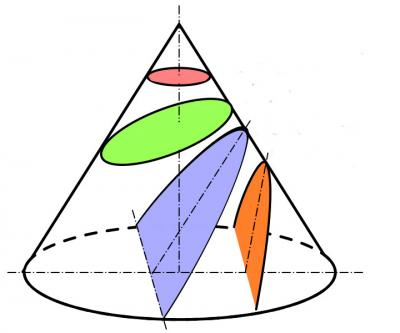
\includegraphics[width=.5\textwidth]{cone_intersection.jpg}
\end{figure}
Якщо площина паралельна основі конуса, то перетин - коло.\\
Якщо площина нахилена основі конуса, то перетин - еліпс.\\
Якщо площина нахилена так, що вона паралельна твірної, то перетин - парабола.\\
Якщо площина ще сильніше нахилена, то перетин - гіпербола.


\subsection{Поверхні другого роду}
\begin{definition}
\textbf{Загальне рівняння поверхні другого порядку} визначається такою формулою:
\begin{align*}
a_{11}x^2 + a_{22}y^2 + a_{33}z^2 + 2a_{12}xy + 2a_{13}xz + 2a_{23}yz + b_1x + b_2y + b_3z + c = 0
\end{align*}
\end{definition}

\begin{lemma}
Задано точку $M_0 = (x_0,y_0)$. При обертанні цієї точки навколо вісі $OX$ отримуємо коло, яке задається рівнянням:\\
$\begin{cases}
x = x_0 \\
y^2 + z^2 = y_0^2
\end{cases}
$\\
\textit{Думаю, тут все зрозуміло}.
\begin{figure}[H]
\centering
\begin{tikzpicture}
%plane
\draw[fill] (0.5,0,0.5) circle (1pt) node [anchor = north]{$M_0$};

\draw[thick, ->] (0,0,0)--(2,0,0) node[anchor = north, black] {$y$};
\draw[thick, ->] (0,0,0)--(0,2,0) node[anchor = east] {$z$};
\draw[thick, ->] (0,0,0)--(0,0,2) node[anchor = north east] {$x$};
\draw[dashed] (0,0,0.5) circle (0.5);
\draw[thick, ->] (-2,0.5,-2) arc (0:220:0.5);
\end{tikzpicture}
\end{figure}
\end{lemma}

\begin{lemma}
У площині $XOY$ задана така крива рівнянням $F(x,y)$, що є парною відносно $y$ (тобто крива симетрична відносно $OY$). При обертанні цієї кривої навколо осі $OX$ отримуємо поверхню, яка задається рівнянням:\\
$F(x,\sqrt{y^2+z^2})=0$.
\end{lemma}

\begin{proof}
Фіксуємо $M_0 = (x_0,y_0)$ - точку кривої. Зробимо обертання навколо $OX$, тоді отримаємо коло:\\
$\begin{cases}
x = x_0 \\
y^2 + z^2 = y_0^2
\end{cases}
$\\
Звідси $|y_0| = \sqrt{y^2+z^2}$. Для т. $x_0,y_0$ виконана рівність:\\
$F(x_0,y_0) = F(x_0, \sqrt{y^2+z^2}) = 0$.\\
Але т. $M_0$ була довільною, тому $F(x,\sqrt{y^2+z^2})=0$, що й є бажаною поверхнею.
\end{proof}

\subsubsection{Еліпсоїд}
У нас вже є еліпс $\dfrac{x^2}{a^2} + \dfrac{y^2}{b^2} = 1$. Обернемо його навколо $OX$, тоді отримуємо:\\
$\dfrac{x^2}{a^2} + \dfrac{y^2+z^2}{b^2} = 1$\\
Отримаємо еліпсоїд обертання:\\
$\dfrac{x^2}{a^2} + \dfrac{y^2}{b^2} + \dfrac{z^2}{b^2} = 1$\\
Зробимо стискання/розтягнення вздовж осі $OZ$, тобто $z_{old} = \lambda z_{new}$. Тобто $\dfrac{z^2}{b^2} \to \dfrac{\lambda^2 z^2}{b^2} = \dfrac{z^2}{c^2}$.\\
Отримаємо \textbf{канонічне рівняння еліпсоїда:}
\begin{align*}
\dfrac{x^2}{a^2} + \dfrac{y^2}{b^2} + \dfrac{z^2}{c^2} = 1
\end{align*}
\begin{figure}[H]
\centering
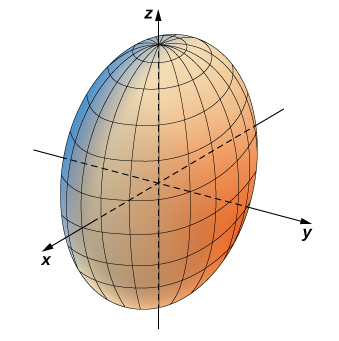
\includegraphics[scale=1]{ellipsoid.jpeg}
\end{figure}
%
%\begin{tikzpicture}[scale = 1.5]
%\draw[->] (0,0,0) -- (2.5,0,0)node[below]{$y$};
%\draw[->] (0,0,0) -- (0,1.5,0)node[left]{$z$};
%\draw[->] (0,0,0) -- (0,0,3)node[left]{$x$};
%\draw[pattern = north east lines, pattern color = red, dashed] (-0.8,0,0) ellipse (0.3 and {sqrt(1 - 0.8*0.8/4)});
%\draw[color=red] (0,0,0) ellipse (2cm and 1cm);
%\draw[color = red, dashed](2,0,0) arc (0:180: 2cm and 0.5cm);
%\draw[color = red](-2,0,0) arc (180:360: 2cm and 0.5cm);
%\node at (2,0,0) [anchor = north west] {$b$};
%\node at (0,1,0) [anchor = south west] {$c$};
%\node at (0,0,2.3) [anchor = east] {$a$};
%\end{tikzpicture}

\subsubsection{Гіперболоїд}
I. Візьмемо гіперболу $\dfrac{z^2}{c^2} - \dfrac{x^2}{a^2} = 1$. Обернемо навколо $OZ$, тоді отримаємо:\\
$\dfrac{z^2}{c^2} - \dfrac{x^2+y^2}{b^2} = 1$.\\
Отримаємо гіперболоїд обертання:\\
$\dfrac{z^2}{c^2} - \dfrac{x^2}{b^2} - \dfrac{y^2}{b^2} = 1$\\
Зробимо стискання/розтягнення вздовж осі $OX$, тобто $x_{old} = \lambda x_{new}$. Тобто $\dfrac{x^2}{b^2} \to \dfrac{\lambda^2 x^2}{b^2} = \dfrac{x^2}{a^2}$.\\
Отримаємо \textbf{канонічне рівняння двопорожнинного гіперболоїда:}
\begin{align*}
\dfrac{z^2}{c^2} - \dfrac{x^2}{a^2} - \dfrac{y^2}{b^2} = 1
\end{align*}
\begin{figure}[H]
\centering
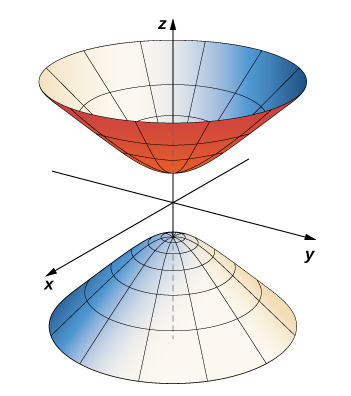
\includegraphics[scale=1]{2-shit-hyperboloid.jpeg}
\end{figure}

II. Візьмемо гіперболу $\dfrac{x^2}{a^2} - \dfrac{z^2}{c^2} = 1$. Обернемо навколо $OZ$, тоді отримаємо:\\
$\dfrac{x^2+y^2}{a^2} - \dfrac{z^2}{c^2} = 1$\\
$\dfrac{x^2}{a^2} + \dfrac{y^2}{a^2} - \dfrac{z^2}{c^2} = 1$\\
Зробимо стискання/розтягнення вздовж осі $OY$, тобто $y_{old} = \lambda y_{new}$. Тобто $\dfrac{y^2}{a^2} \to \dfrac{\lambda^2 y^2}{a^2} = \dfrac{y^2}{b^2}$\\
Отримаємо \textbf{канонічне рівняння однопорожнинного гіперболоїда:}
\begin{align*}
\dfrac{x^2}{a^2} + \dfrac{y^2}{b^2} - \dfrac{z^2}{c^2} = 1
\end{align*}

\begin{figure}[H]
\centering
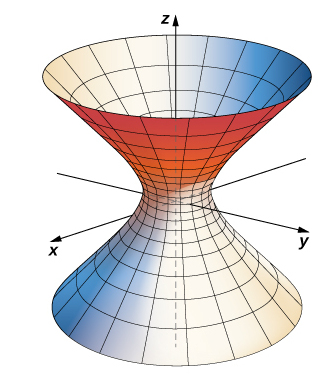
\includegraphics[scale=1]{1-shit-hyperboloid.jpeg}
\end{figure}

\subsubsection{Параболоїд}
У нас вже є парабола $y^2 = 4px$. Обернемо навколо $OX$, тоді отримаємо:\\
$y^2+z^2 = 4px \implies x = \dfrac{y^2}{4p} + \dfrac{z^2}{4p}$.\\
Знову ті махінації з $OZ$, а також $z \to x$.\\
I. Отримаємо \textbf{рівняння еліптичного параболоїду:}
\begin{align*}
z = \dfrac{x^2}{a^2} + \dfrac{y^2}{b^2}
\end{align*}
\begin{figure}[H]
\centering
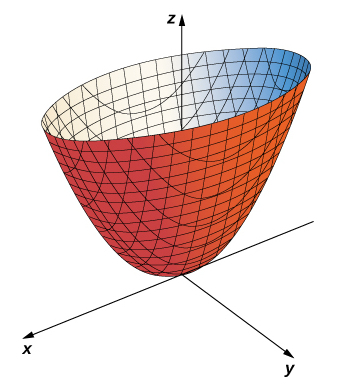
\includegraphics[scale=1]{elliptic-paraboloid.jpeg}
\end{figure}
II. Також отримаємо \textbf{рівняння гіперболічного параболоїду:}
\begin{align*}
z = \dfrac{x^2}{a^2} - \dfrac{y^2}{b^2}
\end{align*}

\begin{figure}[H]
\centering
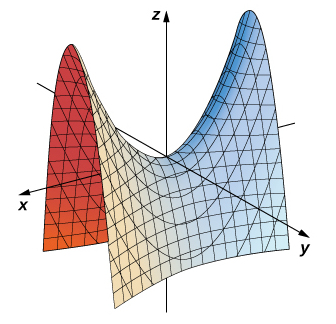
\includegraphics[scale=1]{hyperbolic-paraboloid.jpeg}
\end{figure}

\subsection{Циліндри}
На площині $XOY$ задана крива $F(x,y) = 0$ - основа циліндра - та пряма $l$, що перетинає основу. Через кожну точку основи $M = (x,y,0)$ проведемо пряму, паралельну $l$.\\
Отримана множина точок і є \textbf{циліндром} із основою $F(x,y) = 0$ та прямою $l$.\\

\subsubsection{Еліптичний циліндр}
$\vec{l} = (0,0,1)$\\
$\dfrac{x^2}{a^2} + \dfrac{y^2}{b^2} = 1$\\
Будь-яка точка, що належить еліпсу, буде належати циліндру.

\subsubsection{Гіперболічний циліндр}
$\vec{l} = (0,0,1)$\\
$\dfrac{x^2}{a^2} - \dfrac{y^2}{b^2} = 1$\\
Будь-яка точка, що належить гіперболі, буде належати циліндру.

\subsubsection{Параболічний циліндр}
$\vec{l} = (0,0,1)$\\
$y^2 = 4px$\\
Будь-яка точка, що належить параболі, буде належати циліндру.

\subsection{Конічні поверхні}
На площині $XOY$ задана крива $F(x,y) = 0$ - основа конуса - та пряма $l$, що перетинає основу. Через кожну точку основи $M = (x,y,0)$ проведемо пряму, паралельну $l$.\\
Отримана множина точок і є \textbf{циліндром} із основою $F(x,y) = 0$ та т. $K = (x_k, y_k, \underset{\neq 0}{z_k})$ - вершина конусу. Проведемо прямі, які проходять через вершину конусу $K$ та через основу\\
Отримана множина точок і є \textbf{конусом} із основою $F(x,y) = 0$ та вершиною $K = (x_k, y_k, \underset{\neq 0}{z_k})$.

\subsubsection*{Вироджені поверхні другого роду}
I. $\dfrac{x^2}{a^2} + \dfrac{y^2}{b^2} + \dfrac{z^2}{c^2} = 0$ - точка.\\
II. $\dfrac{x^2}{a^2} + \dfrac{y^2}{b^2} + \dfrac{z^2}{c^2} = -1$ - уявний еліпсоїд.\\
III. $(A_1 x + B_1 y + C_1 z + D_1)(A_2 x + B_2 y + C_2 z + D_2) = 0$ - пара площин.
\newpage

\section{Многочлени}
\begin{definition}
\textbf{Многочленом} називають функцію такого вигляду:
\begin{align*}
P_n(x) = a_0 + a_1 x + \dots + a_n x^n,
\end{align*}
де $a_0,a_1,\dots,a_n \in \mathbb{R}$ або $\mathbb{C}$ (або будь-яке інше поле $k$).\\
Для них все зрозуміло з операціями додавання та множення многочлена на скаляр.\\
Позначення: $\mathbb{R}[x]$ - клас многочленів з дійсними коефіцієнтами.
\end{definition}

\begin{definition}
\textbf{Степенем} многочлена $f(x) = a_0 + a_1 x + \dots + a_n x^n$ називають найвищий степінь із всіх одночленів.\\
Позначення: $\deg f$.
\end{definition}

\begin{example}
Зокрема для многочлена $f(x) = x^2 + 1$ маємо $\deg f = 2$.
\end{example}

\subsection{Про подільність многочленів}
\begin{theorem}
Для будь-яких многочленів $f(x)$ та $g(x)$ існують \textit{єдині} многочлени $s(x)$, $r(x)$, для яких $f(x) = s(x) g(x) + r(x)$,\\
де $\deg r < \deg g$ або $r \equiv 0$.
\end{theorem}

\begin{proof}
\textit{Існування.}\\
Маємо якісь многочлени $f,g$. Тут є два випадки.
I. $\deg f < \deg g$. Тоді $s(x) = 0$ та $r(x) = f(x)$. Отримали те, що потрібно було.
\bigskip \\
II. $\deg f \geq \deg g$. Проведемо МІ за числом $\deg f -\deg g = k$.\\
База індукції. $k = 0$, тобто $\deg f = \deg g \overset{\text{позн.}}{=} n$.
Тож маємо такі многочлени:\\
$f(x) = a_n x^n + \dots + a_0$;\\
$g(x) = b_n x^n + \dots + b_0$.\\
Перепишемо многочлен $f$ під той лад, що ми хочемо:\\
$f(x) = \underbrace{\dfrac{a_n}{b_n}}_{=s(x)} (b_n x^n + \dots + b_0) + \underbrace{\left(a_{n-1}x^{n-1}+\dots+a_0 - \dfrac{a_n b_{n-1}}{b_n}x^{n-1}- \dots - \dfrac{b_0 a_n}{b_n} \right)}_{= r(x)}$.\\
Важливо зауважити, що тут $\deg r =n-1 < n = \deg g$. Базу індукції довели.
\bigskip \\
Крок індукції. Нехай для $k \geq 0$ теорема виконується, тобто існують $\tilde{s}(x), \tilde{r}(x)$.
\bigskip \\
Доведемо існування $s(x)$ та $r(x)$ для випадку $k+1$. Нехай $\deg f = k+1+m$, тоді $\deg g = m$.\\
$f(x) = a_{m+k+1} x^{m+k+1} + a_{m+k}x^{m+k} + \dots + a_0$;\\
$g(x) = b_m x^m + \dots + b_0$.\\
Приблизно аналогічним чином ми перепишемо $f$ під наш лад:\\
$f(x) = \dfrac{a_{m+k+1}}{b_m}x^{k+1} (b_m x^m + \dots + b_0)
+ \underbrace{\left(a_{m+k}x^{m+k} + \dots + a_0 - \left(\dfrac{b_{m-1}a_{m+k+1}}{b_m}x^{m+k} + \dots + \dfrac{b_0 a_{m+k+1}}{b_m}x^k \right) \right)}_{=p(x)}$\\
$f(x) = \dfrac{a_{m+k+1}}{b_m}x^{k+1}g(x) + p(x)$.\\
Зауважимо у цьому випадку, що $\deg p = m+k < m+k+1 = \deg f$. Також $\deg p - \deg g = k$, тож за припущеннями МІ, для многочленів $p(x),g(x)$ існує $\tilde{s}(x), \tilde{r}(x)$, для яких $p(x) = \tilde{s}(x) g(x) + \tilde{r}(x)$. Звідси\\
$f(x) = \dfrac{a_{m+k+1}}{b_m}x^{k+1}g(x) + \tilde{s}(x)g(x) + \tilde{r}(x) = \underbrace{\left(\dfrac{a_{m+k+1}}{b_m}x^{k+1} + \tilde{s}(x) \right)}_{=s(x)}g(x) + \underbrace{\tilde{r}(x)}_{=r(x)}$.\\
Зауважимо, що $\deg r < \deg g$ (припущення МІ) або $r \equiv 0$.\\
МІ доведено.
\bigskip \\
\textit{Єдиність.}\\
!Припустимо, що крім $s,r$ існують ще $s^*,r^*$, такі, що також $f(x) = s^*(x)g(x) + r^*(x)$. Причому $\deg r^* < \deg g$ або $r^* \equiv 0$. Тоді \\ $0 = f(x) - f(x) = (s(x)-s^*(x))g(x) + (r(x)-r^*(x))$.\\
$(s(x)-s^*(x))g(x) = r^*(x)-r(x)$, де $\deg(r^*-r) < \deg g$. Із цієї оцінки випливає, що рівність можлива лише тоді, коли $s(x)-s^*(x) =0 \implies s(x) = s^*(x)$.\\
А звідси й $r(x) = r^*(x)$. Суперечність!
\end{proof}

\begin{example}
Зокрема $x^2-2 = (x-1)(x+1) -1$.\\
Тут ніби ми ділили $x^2-2$ на $x-1$, тоді отримаємо $x+1$ з остачею $-1$.
\end{example}

\subsection{Корені многочленів}
\begin{definition}
Число $a$ називають \textbf{коренем многочлена} $f(x)$, якщо
\begin{align*}
f(a) = 0
\end{align*}
\end{definition}

\begin{theorem}[Теорема Безу]
Остача ділення многочлена $f(x)$ на многочлен $x-a$ дорівнює $f(a)$.
\end{theorem}

\begin{proof}
Дійсно, маємо $f(x) = s(x)(x-a) + r(x)$, причому $\deg r < \deg (x-a) = 1$. Тому єдиний варіант - це бути $r(x) = c, c \in \mathbb{R}$.\\
Отже, $f(x) = s(x)(x-a) + c$. Нарешті, підставимо $x = a$ - отримаємо $f(a) = c$. Отже,\\
$f(x) = s(x)(x-a) + f(a)$.
\end{proof}

\begin{corollary}
$a$ - корінь многочлена $f(x) \iff \exists h: f(x) = (x-a)h(x)$.\\
\textit{Думаю, зрозуміло.}
\end{corollary}

\begin{definition}
Число $a$ називають \textbf{коренем многочлена} $f(x)$ \textbf{кратності} $k$, якщо 
\begin{align*}
f(x) = (x-a)^k g(x),
\end{align*}
причому вимагається $g(a) \neq 0$.\\
Іншими словами, $(x-a)^k \mid f$, але $(x-a)^{k+1} \nmid f$.
\end{definition}

\subsection*{Розклад многочлена за степенем лінійного двочлена}
Перед однією теоремою зауважимо наступне. Маємо многочлен\\
$f(x) = a_0 + a_1 x + \dots + a_n x^n$.\\
Хочеться переписати його в іншому вигляді. Замість $x$ хочеться всюди $x-a$.\\
За теоремою Безу, маємо $f(x) = (x-a)s_1(x) + f(a)$. Тут обов'язково $\deg s_1 = n-1$. Для спрощення позначу $f(a) = c_0$.\\
Знову за теоремою Безу, маємо $f(x) = (x-a)((x-a)s_2(x) + s_1(a)) + c_0 = (x-a)^2 s_2(x) + c_1 (x-a) + c_0$, тут $c_0 = s_1(a)$. Обов'язково $\deg s_2 = n-2$.\\
Знову за теоремою Безу, маємо $f(x) = (x-a)^2 ((x-a)s_3(x) + s_2(a)) + c_1(x-a) + c_0 = (x-a)^3 s_3(x) + c_2 (x-a)^2 + c_1(x-a) + c_0$.\\
\vdots \\
Продовжуємо цей процес, допоки $\deg s_{\text{деякий}} = 1$, отримаємо\\
$f(x) = c_0 + c_1 (x-a) + c_2 (x-a)^2 + \dots + c_{n-2}(x-a)^{n-2} + s_{n-1}(x) (x-a)^n$.\\
Останній раз беремо Безу, отримаємо $s_{n-1}(x) = (x-a) c_n + c_{n-1}$, де $c_{n-1} = s_{n-1}(a)$.\\
Разом отримали таку форму:
\begin{align*}
f(x) = c_0 + c_1(x-a) + c_2(x-a)^2 + \dots + c_n(x-a)^n
\end{align*}
Тепер питання полягає в тому, як знайти $c_0,c_1,\dots,c_n$. Ми вже знаємо, що многочлен - диференційована функція, тому можемо знайти коефіцієнти через похідні таким чином:\\
$\begin{cases}
f(a) = c_0\\
f'(a) = 1!c_1\\
f''(a) = 2!c_2\\
\vdots \\
f^{(n)}(a) = n!c_n
\end{cases} \implies c_k = \dfrac{f^{(k)}(a)}{k!}, k = \overline{0,n}$.\\
Отже, отримали більш красиву форму:
\begin{align*}
f(x) = f(a) + \dfrac{f'(a)}{1!}(x-a) + \dots + \dfrac{f^{(n)}(a)}{n!}(x-a)^n
\end{align*}
Права частина має особливу назву - \textbf{многочлен Тейлора}.
\bigskip \\
\textbf{Повернімось до попереднього розділу.}
\begin{theorem}[Критерій кратності кореня]
$a$ - корінь кратності $k$ многочлена $f(x) \iff f(a)=f'(a)=\dots=f^{(k-1)}(a) =0$, але $f^{(k)}(a) \neq 0$.
\end{theorem}

\begin{proof}
\rightproof Дано: $a$ - корінь кратності $k$ для $f(x)$, тобто $f(x) = (x-a)^k g(x)$, де $g(a) \neq 0$.\\
Ба більше, якщо $\deg f = n$, то звідси $\deg g = n-k$. Тому розкладемо функцію $g$ за щойно отриманою формулою:\\
$f(x) = (x-a)^k \left(g(a) + \dfrac{g'(a)}{1!}(x-a) + \dots + \dfrac{g^{(n-k)}(a)}{(n-k)!}(x-a)^{n-k} \right) = \\
= (x-a)^k g(a) + (x-a)^{k+1}\dfrac{g'(a)}{1!} + \dots + (x-a)^n\dfrac{g^{(n+k)}(a)}{(n+k)!}$\\
Але з іншого боку,\\
$f(x) = f(a) + \dfrac{f'(a)}{1!}(x-a) + \dots + \dfrac{f^{(k-1)}(a)}{(k-1)!}(x-a)^{k-1} + \dfrac{f^{(k)}(a)}{k!}(x-a)^{k} + \dots + \dfrac{f^{(n)}(a)}{n!}(x-a)^n$\\
В першому рівності многочлен починався зі степені $k$, тому й друга рівність має починатись зі степені $k$, звідси й\\
$f(a) = 0 \hspace{0.5 cm} \dfrac{f'(a)}{1!} = 0 \hspace{0.5 cm} \dots \hspace{0.5 cm} \dfrac{f^{(k-1)}(a)}{k!} = 0$\\
При цьому $\dfrac{f^{(k)}(a)}{k!} \neq 0$. Отже, отримали бажану умову.
\bigline
\leftproof Дано: $f(a)=f'(a)=\dots=f^{(k-1)}(a) =0$, але $f^{(k)}(a) \neq 0$.\\
Розкладемо нашу функцію $f$ за формулою:\\
$f(x) = f(a) + \dfrac{f'(a)}{1!}(x-a) + \dots \dfrac{f^{(k-1)}(a)}{(k-1)!}(x-a)^{k-1} + \dfrac{f^{(k)}(a)}{k!}(x-a)^{k} + \dots + \dfrac{f^{(n)}(a)}{n!}(x-a)^n$\\
Тоді\\
$f(x) = \dfrac{f^{(k)}(a)}{k!}(x-a)^{k} + \dots + \dfrac{f^{(n)}(a)}{n!}(x-a)^n = (x-a)^k \underbrace{\left(\dfrac{f^{(k)}(a)}{k!} + \dots + \dfrac{f^{(n)}(a)}{n!}(x-a)^{n-k} \right)}_{=g(x)}$.\\
Через те, що $f^{(k)}(a) \neq 0$, то звідси $g(a) \neq 0$. Отже, $f(x) = (x-a)^k g(x) \Rightarrow$ $a$ - корінь кратності $k$.
\end{proof}

\subsection{Комплексні корені многочленів}
\begin{proposition}
Якщо $z \in \mathbb{C}$ є коренем многочлена $f(x)$ з дійсними коефіцієнтами, то $\bar{z}$ - теж корінь многочлена $f(x)$.
\end{proposition}

\begin{proof}
Задано многочлен $f(x) = a_n x^n + \dots + a_0$, для якого $f(z) = 0$. Тоді маємо:\\
$f(\bar{z}) = a_n \bar{z}^n + \dots + a_0 = \overline{a_n z^n} + \dots + \overline{a_0} = \overline{a_n z^n + \dots + a_0} = \overline{f(z)} = \bar{0} = 0$
\end{proof}

\begin{proposition}
Корені $z$ та $\bar{z}$ мають однакову кратність.
\end{proposition}

\begin{proof}
Нехай $z$ - корінь кратності $k$, тобто $f(z) = f'(z) = \dots = f^{(k-1)}(z) = 0, f'^{(k)}(z) \neq 0$.\\
Тоді за міркуваннями попереднього твердження, і$f(\bar{z}) = f'(\bar{z}) = \dots = f^{(k-1)}(\bar{z}) = 0, f'^{(k)}(\bar{z}) \neq 0$. \\ Отже, $\bar{z}$ - корінь кратності $k$.
\end{proof}

\begin{theorem}[Основна теорема алгебри]
У многочлена з комплексними коефіцієнтами є принаймні один корень $z_0 \in \mathbb{C}$.\\
\textit{Без доведення.}\\
\textit{А все тому, що доведення або вимагає знання комплексного аналізу, або треба вчити спеціальні розділи математики. Простого доведення нема.}
\end{theorem}

\begin{corollary}
Задано многочлен степені $n$ з комплексними коефіцієнтами. Тоді многочлен має рівно $n$ коренів, враховуючи кратність.
\end{corollary}

\begin{proof}
Нехай (за основною теоремою алгебри) $z_1$ - корінь $f(z) \implies f(z) = (z-z_1)^{k_1} g(z)$, причому $g(z_1) \neq 0$.\\
За основною теоремою алгебри, $g(z)$ має корінь $z_2 \implies g(z) = (z-z_2)^{k_2} g_2(z)$, причому $g_2(z_2) \neq 0$.\\
І знову за основною теоремою алгебри, $g_2(z)$ має корінь $z_3\dots$\\
Продовжуючи до кінця, отримуємо остаточно:\\
$f(z) = A_0(z-z_1)^{k_1}(z-z_2)^{k_2}\dots(z-z_m)^{k_m}$, де \hspace{0.5cm} $k_1 + k_2 + \dots + k_m = n = \deg f$.
\end{proof}

\begin{theorem}
Функція $f(x)$ з дійсними коефіцієнтами розкладається на такі прості множники:\\
$f(x) = A_0 (x-a_1)^{k_1} \dots (x-a_m)^{k_m} (x^2+p_1x+q_1)^{s_1} \dots (x^2+p_j+q_j)^{s_j}$, де \\
$k_1 + \dots + k_m + 2s_1 + \dots + 2s_j = n = \deg f$.\\
Тут $A_0, a_1,\dots,a_m, p_1,q_1,\dots,p_j,q_j \in \mathbb{R}$.\\
Ба більше, всі дискримінанти квадратних рівнянь - від'ємні.
\end{theorem}

\begin{proof}
За попереднім наслідком,\\
$f(x) = A_0(x-a_1)^{k_1} \dots (x-a_m)^{k_m} (x-z_1)^{s_1} (x-\bar{z_1})^{s_1} \dots (x-z_j)^{s_j} (x-\bar{z_j})^{s_j}$\\
Розпишемо такі добутки:\\
$(x-z_1)(x-\bar{z_1}) = x^2 - x(z_1 +\bar{z_1}) + z_1 \bar{z_1} \boxed{=}$\\
$z_1 + \bar{z_1} = 2 \Re z_1 \overset{\textrm{позн.}}{=} -p_1 \in \mathbb{R}$\\
$z_1 \bar{z_1} = |z|^2 \overset{\textrm{позн.}}{=} q_1 \in \mathbb{R}$\\
$\boxed{=} x^2 + p_1x + q_1$, для якого $D < 0$. Бо мали справу з комплексними коренями.\\
І так з рештою. Тому\\
$f(x) = A_0 (x-a_1)^{k_1} \dots (x-a_m)^{k_m} (x^2+p_1x+q_1)^{s_1} \dots (x^2+p_j+q_j)^{s_j}$
\end{proof}

\subsection{Спільні дільники та кратні двох многочленів}
\begin{definition}
Многочлен $h(x)$ називається \textbf{дільником} многочлена $f(x)$, якщо
\begin{align*}
\exists s(x): f(x) = s(x) h(x)
\end{align*}
Позначення: $h \mid f$.
\end{definition}

\begin{definition}
Многочлен $d(x)$ називається \textbf{спільним дільником} многочленів $f(x)$ та $g(x)$, якщо
\begin{align*}
d \mid f \hspace{1cm} d \mid g
\end{align*}
\end{definition}

\begin{definition}
Многочлен $D(x)$ називається \textbf{найбільшим спільним дільником} многочленів $f(x),g(x)$, якщо
\begin{align*}
\forall d - \text{спільний дільник }f,g: d \mid D
\end{align*}
Позначення: $D = \gcd(f,g)$.
\end{definition}

\begin{corollary}
Нехай $d$ - довільний дільник многочленів $f,g$.\\
Тоді $\deg d \leq \deg \gcd(f,g)$.\\
\textit{Відносно зрозуміло.}
\end{corollary}

\begin{proposition}
Нехай $D_1, D_2$ - два найбільших спільних дільника многочленів $f,g$.\\
Тоді $\exists c \in \mathbb{R}: D_1(x) = c D_2(x)$.
\end{proposition}

\begin{proof}
Якщо $D_1(x) = \gcd(f,g) (x)$ та $D_2$ - спільний дільник $f,g$, то $D_2 \mid D_1$, тобто $D_1(x) = s_1(x) D_2(x)$.\\
Якщо $D_2(x) = \gcd(f,g) (x)$ та $D_1$ - спільний дільник $f,g$, то $D_1 \mid D_2$, тобто $D_2(x) = s_2(x) D_1(x)$.\\
Друге рівняння підставимо в перше - отримаємо:\\
$D_1(x) = s_1(x) D_2(x) = s_1(x)s_2(x)D_1(x)$\\
$\implies s_1(x)s_2(x) = 1 \implies s_1(x) = c_1, s_2(x) = c_2 = \dfrac{1}{c_1}$.\\
Отже, $D_1(x) = c_1 D_2(x)$.
\end{proof}

Отже, всі найбільші спільні дільники між многочленами $f,g$ рівні з точністю до деякої константи.

\begin{theorem}[Алгоритм Евкліда]
Задані многочлени $f,g$. Запишемо ділення з остачею таким чином:\\
$\begin{cases}
f(x) = s_1(x) g(x) + r_1(x) \\
g(x) = s_2(x) r_1(x) + r_2(x) \\
r_1(x) = s_3(x) r_2(x) + r_3(x) \\
\vdots \\
r_{n-2}(x) = s_n(x)r_{n-1}(x) + r_n(x) \\
r_{n-1}(x) = s_{n+1}(x) r_n(x)
\end{cases}$.\\
Тоді $\gcd(f,g) = r_n(x)$, тобто останній ненульовий остача-многочлен.
\end{theorem}

\begin{remark}
Алгоритм Евкліда має скінченне число ітерацій, просто тому що\\
$\deg f > \deg g > \deg r_1 > \deg r_2 > \dots > \deg r_n$.\\
У силу строгої нерівності рано чи пізно буде остача-многочлен $0$.
\end{remark}

\begin{proof}
Покажемо, що $r_n(x)$ - спільний дільник $f,g$.\\
Дійсно, якщо $r_{n-1}$ підставити в останнє рівняння, потім $r_{n-2}$ в передостаннє і так до кінця, то отримаємо, що спочатку $r_n \mid g$, а якщо підставити $g$ в найперше рівняння, то $r_n \mid f$.\\
Покажемо, що $r_n(x)$ - найбільший спільний дільник $f,g$.\\
Дійсно, якщо $d$ - довільний спільний дільник $f,g$, то звідси $d \mid r_1, d \mid r_2, \dots, d \mid r_n$. Це доводиться, якщо йти згори вниз поступово.\\
Таким чином, $r_n(x) = \gcd(f,g)$.
\end{proof}

\iffalse
\begin{definition}
Многочлен $l(x)$ називається \textbf{спільним кратним} многочленів $f(x)$ та $g(x)$, якщо
\begin{align*}
f | l \hspace{1cm} g | l
\end{align*}
\end{definition}

\begin{definition}
Многочлен $L(x)$ називається \textbf{найменшим спільним кратним} многочленів $f(x),g(x)$, якщо:
\begin{align*}
\forall l - \text{ спільне кратне } f,g: L | l
\end{align*}
Позначення: $L = \lcm(f,g)$.
\end{definition}

\begin{theorem}
$\gcd (f,g) \cdot \lcm (f,g) = f(x)g(x)$.
\end{theorem}

\begin{proof}
Маємо $D(x) = \gcd(f,g)$, тобто звідси $D | f, D | g \implies f(x) = f_1(x)D(x), g(x) = g_1(x)D(x)$.\\
Розглянемо многочлен $L(x) = f_1(x)g_1(x)D(x)$. Це буде спільним кратним $f,g$. Дійсно,\\
$L(x) = f(x)g_1(x) \implies f | L$\\
$L(x) = g(x)f_1(x) \implies g | L$.\\
Оберемо будь-яке спільне кратне $l$ многочленів $f,g$. Тоді звідси $l(x) = f(x) u(x)$ та $l(x) = g(x) v(x)$.\\
\end{proof}

\defin{5.3.5.(1)} Многочлен $m(x)$ називається \textbf{спільним кратним} $f(x)$ та $g(x)$, якщо $m(x)$ ділиться на $f(x)$ та $g(x)$ одночасно
\bigline
\defin{5.3.5.(2)} Многочлен $M(x)$ називається \textbf{\underline{найменшим} спільним кратним} $f(x)$ та $g(x)$, якщо він ділиться без остачі на будь-яке спільне кратне $f(x)$ та $g(x)$\\
Позначення: $M(x) = \textrm{LCM}(f,g)$
\bigline
\textbf{Знаходження НСК}\\
I. Знайти $\textrm{GCD}(f,g) = d(x)$, тобто\\
$f(x) = f_1(x) d(x)$\\
$g(x) = f_2(x) d(x)$\\
II. Тоді $k(x) = f_1(x)f_2(x)d_2(x)$\\
Це є спільним кратним $f(x)$ та $g(x)$\\
Будь-яке спільне кратне повинно ділитись на $f(x)$ та $g(x)$, а отже, й на $f_1(x)f_2(x)d(x) = k(x)$\\
Звідси отримуємо\\
$\textrm{LCM}(f,g) = \dfrac{f(x)g(x)}{\textrm{GCD}(f,g)}$
\bigline
\prp{5.3.6.} Нехай $k_1$ та $k_2$ - НСК $f(x)$ та $g(x)$\\
Тоді $\exists c \in \mathbb{R}: k_1(x) = ck_2(x)$\\
\proof
Скористаємось отриманою щойно формулою\\
Коли $k_1(x) = \textrm{LCM}(f,g)$, то $d_1(x) = \textrm{GCD}(f,g) = \dfrac{f(x)g(x)}{k_1(x)}$\\
Коли $k_2(x) = \textrm{LCM}(f,g)$, то $d_2(x) = \textrm{GCD}(f,g) = \dfrac{f(x)g(x)}{k_2(x)}$\\
Але оскільки $d_1(x) = c^*d_2(x)$, то звідси $\dfrac{1}{k_1(x)} = \dfrac{c^*}{k_2(x)} \Rightarrow k_1(x) = c k_2(x)$ \qed
\bigline
\fi

\subsection{Дробово-раціональні вирази, розклад}
\begin{definition}
\textbf{Дробово-раціональним виразом} називають дріб $\dfrac{P(x)}{Q(x)}$, де $P(x),Q(x)$ - многочлени.
\end{definition}

\begin{definition}
\textbf{Простими дробами} називають один із дробово-раціональних виразів
\begin{align*}
\dfrac{1}{x-a} \hspace{1cm} \dfrac{1}{(x-a)^k} \hspace{1cm} \dfrac{Ax+B}{x^2+px+q} \hspace{1cm} \dfrac{Ax+B}{(x^2+px+q)^k}
\end{align*}
Останні два дроби - це в дійсному випадку. Ба більше, дискриминанти знаменників - від'ємні.
\end{definition}

\subsubsection*{Розклад дробово-раціональних виразів на суму простих дробів}
I. $\deg P \geq \deg Q$.\\
У цьому випадку ми ділимо $P$ на $Q$ (стовпчиком), тоді отримаємо:\\
$P(x) = S(x)Q(x) + P_1(x)$.\\
Звідси $\dfrac{P(x)}{Q(x)} = S(x) + \dfrac{P_1(x)}{Q(x)}$. Але ось тут вже $\deg P_1  < \deg Q$. Зараз ми розглянемо це випадок окремо.
\bigskip \\
II. $\deg P < \deg Q$.\\
У такому разі дріб $\dfrac{P(x)}{Q(x)}$ називають \textbf{правильним}.
Уже відомо, що можна розкласти $Q(x) = E(x-a_1)^{k_1} \dots (x-a_m)^{k_m} (x^2+p_1x+q_1)^{l_1} \dots (x^2+p_s x+q_s)^{l_s}$ саме таким чином.

\begin{lemma}
Задано $\dfrac{P(x)}{Q(x)}$ - такий дробово-раціональний вираз, що $\deg P < \deg Q$. Відомо, що $Q(x) = (x-a)^k Q_1(x)$, де $Q_1(a) \neq 0$.\\
Тоді $\exists A \in \mathbb{R}, \exists P_1(x): \deg P_1 < \deg P$, для яких можемо записати\\
$\dfrac{P(x)}{Q(x)} = \dfrac{A}{(x-a)^k} + \dfrac{P_1(x)}{(x-a)^{k-1}Q_1(x)}$.
\end{lemma}

\begin{proof}
Хочемо знайти $A$ та $P_1(x)$, для яких виконується рівність:\\
$\dfrac{P(x)}{(x-a)^kQ_1(x)} = \dfrac{A}{(x-a)^k} + \dfrac{P_1(x)}{(x-a)^{k-1}Q_1(x)}$.\\
$\dfrac{P(x)}{(x-a)^k Q_1(x)} = \dfrac{AQ_1(x)+P_1(x)(x-a)}{(x-a)^kQ_1(x)}$.\\
$P(x) = AQ_1(x) + P_1(x)(x-a)$. Причому дана рівність виконується $\forall x \in \mathbb{R}$.\\
Зокрема для $x=a$ маємо $P(a) = AQ_1(x) \implies A = \dfrac{P(a)}{Q_1(a)}$.\\
Крім того, $P_1(x)(x-a) = P(x) - AQ_1(x)$, а оскліьки $P(a) - AQ_1(a) = 0$, то звідси \\
$P(x) -AQ_1(x) = P_1(x)(x-a)$. Тобто $P_1(x)$ отримується діленням $P(x)-AQ_1(x)$ на $(x-a)$.
\end{proof}

\begin{corollary}
$\dfrac{P(x)}{Q_1(x)(x-a)^k} = \dfrac{A_k}{(x-a)^k} + \dfrac{A_{k-1}}{(x-a)^{k-1}} + \dots + \dfrac{A_2}{(x-a)^2} + \dfrac{A_1}{x-a} + \dfrac{R_1(x)}{Q_1(x)}$.\\
У цьому випадку $Q_1(a) \neq 0$.
\end{corollary}

\begin{lemma}
Задано $\dfrac{P(x)}{Q(x)}$ - такий дробово-раціональний вираз, що $\deg P < \deg Q$. Відомо, що $Q(x) = (x^2+px+q)^kQ_1(x)$, де $Q_1(z_0) \neq 0$. Тут в нас $x^2+px+q = (x-z_0)(x+\bar{z_0})$.\\
Тоді $\exists B,C \in \mathbb{R}, \exists P_1(x): \deg P_1 < \deg P$ та $P_1(x)$ не ділиться на $x^2+px+q$, для яких можемо записати\\
$\dfrac{P(x)}{Q(x)} = \dfrac{Bx+C}{(x^2+px+q)^k} + \dfrac{P_1(x)}{(x^2+px+q)^{k-1}Q_1(x)}$.
\end{lemma}

\begin{proof}
Хочемо знайти $B,C$ та $P_1(x)$, для яких виконується рівність:\\
$\dfrac{P(x)}{(x^2+px+q)^k Q_1(x)} = \dfrac{Bx+C}{(x^2+px+q)^k} + \dfrac{P_1(x)}{(x^2+px+q)^{k-1}Q_1(x)}$.\\
$\dfrac{P(x)}{(x^2+px+q)^k Q_1(x)} = \dfrac{(Bx+C)Q_1(x)+P_1(x)(x^2+px+q)}{(x^2+px+q)^k Q_1(x)}$\\
$P(x) = (Bx+C)Q_1(x)+P_1(x)(x^2+px+q)$ $(*)$\\
Нехай $z_0$ та $\bar{z_0}$ - корені $x^2+px+q$. Вони комплексні та спряжені між собою, бо $D < 0$. Ці корені підставимо в наше рівняння (*) - отримаємо ось таку систему:
$\begin{cases} 
P(z_0) = (Bz_0+C)Q_1(z_0) \\
P(\bar{z_0}) = (B\bar{z_0}+C) Q_1(\bar{z_0})
\end{cases}$.\\
Перепишемо обережно в вигляді $\begin{cases} 
P(z_0) = (Bz_0+C)Q_1(z_0) \\
\overline{P(z_0)} = (B\bar{z_0}+C) \overline{Q_1(z_0)}
\end{cases}$.\\
Додамо два рівняння, також віднімемо та поділимо на $i$, тоді:\\
$\begin{cases}
2 \Re P(z_0) = 2B \Re (z_0 Q_1(z_0)) + 2C \Re Q(z_0) \\
2 \Im P(z_0) = 2B \Im(z_0 Q_1(z_0)) + 2C \Im Q(z_0)
\end{cases}
$\\
Ну а далі шукаємо $B,C$, які будуть дійсними числами. Повернімось до рівняння:\\
$P(x) = (Bx+C)Q_1(x) + P_1(x)(x^2+px+q)$. Тут $B,C$ вже маємо. Тоді\\
$P_1(x)(x^2+px+q) = P(x) - (Bx+C)Q_1(x)$.\\
Корені $z_0, \bar{z_0}$ многочлена $x^2+px+q$ є коренями $P(x)-(Bx+C)Q_1(x)$. Тому $P(x) - (Bx+C)Q_1(x)$ ділиться на $x^2+px+q$.\\
Остаточно знайдемо $P_1(x)$ шляхом ділення $P(x) - (Bx+C)Q_1(x)$ на $x^2+px+q$.
\end{proof}

\begin{corollary}
$\dfrac{P(x)}{Q_1(x)(x^2+px+q)^k} = \dfrac{B_kx+C_k}{(x^2+px+q)^k} + \dots + \dfrac{B_2x+C_2}{(x^2+px+q)^2} + \dfrac{B_1x+C_1}{x^2+px+q} + \dfrac{R_1(x)}{Q_1(x)}$.\\
У цьому випадку $Q_1(z_0) \neq 0$ (хоча в дійсному випадку це вимагати не обов'язково).
\end{corollary}

\begin{theorem}
Задано $\dfrac{P(x)}{Q(x)}$ - такий дробово-раціональний вираз, що $\deg P < \deg Q$. Відомо (із наслідку основної теореми алгебри), що \\ $Q(x) = E(x-a_1)^{k_1} \dots (x-a_m)^{k_m} (x^2+p_1x+q_1)^{l_1} \dots (x^2+p_s x+q_s)^{l_s}$. Тоді\\
$E \cdot \dfrac{P(x)}{Q(x)} = \dfrac{A_{11}}{(x-a_1)} + \dots + \dfrac{A_{1k_1}}{(x-a_1)^{k_1}} + \dfrac{A_{21}}{(x-a_2)} + \dots + \dfrac{A_{2k_2}}{(x-a_2)^{k_2}} + \dots + \dfrac{A_{m1}}{(x-a_m)} + \dots + \dfrac{A_{mk_m}}{(x-a_m)^{k_m}} \\ + \dfrac{B_{11}x + C_{11}}{x^2+p_1x+q_1} + \dots + \dfrac{B_{1l_1}x + C_{1l_1}}{(x^2+p_1x+q_1)^{l_1}} + \dots + \dfrac{B_{s1}x + C_{s1}}{x^2+p_s x+q_s} + \dots + \dfrac{B_{sl_s}x + C_{sl_s}}{(x^2+p_s x+q_s)^{l_s}}$\\
\textit{Ґрунтується на основі двох наслідків з двох лем.}
\end{theorem}
$\scaleobj{5}{\blacksquare}$\\
\end{document}
